\documentclass[times, utf8, diplomski]{fer}
\usepackage{booktabs}
\usepackage{listings}
\usepackage{subcaption}
\usepackage{mathtools}
\usepackage{geometry}
\usepackage{amsmath}
\usepackage{array, booktabs, makecell}
\usepackage{siunitx, mhchem}
\DeclarePairedDelimiter\ceil{\lceil}{\rceil}

\lstset{
    numbers=left,
    breaklines=true,
    tabsize=2,
    basicstyle=\ttfamily\scriptsize,
}

\renewcommand{\lstlistingname}{Kod}

\newcommand{\myparagraph}[1]{\paragraph{#1}\mbox{}\\}
\newcommand{\crwd}{\emph{crowdsensing} }

\begin{document}

% % TODO: Navedite broj rada.
% \thesisnumber{000}

% % TODO: Navedite naslov rada.
\title{Stvarnovremenska analiza podataka korisnika javnog gradskog prijevoza}

% % TODO: Navedite svoje ime i prezime.
% \author{Petar Lazić}

% \maketitle

% % Ispis stranice s napomenom o umetanju izvornika rada. Uklonite naredbu \izvornik ako želite izbaciti tu stranicu.
% % \izvornik

% % Dodavanje zahvale ili prazne stranice. Ako ne želite dodati zahvalu, naredbu ostavite radi prazne stranice.
\zahvala{}

\tableofcontents




\chapter{Uvod}

U današnjem svijetu su pametni telefoni sveprisutni, bogati raznim senzorima te gotovo stalno povezani na Internet. 
Te činjenice omogućuju rješavanje nekih problema koristeći usluge grupnog opažanja okoline \engl{mobile crowdsensing}.
Glavna ideja ovog pristupa je prikupljanjem i analizom podataka sa senzora pametnih telefona omogućiti otkrivanje nekih dodatnih informacija koje mogu biti korisne.
Primjeri tih problema za koje već postoje napravljena rješenja su analiza kvalitete zraka (Cupus mobilna aplikacija), analiza gustoće prometa i gužvi (Google maps) te razni drugi.

Problem koji će se razmatrati u ovom radu jest praćenje lokacija vozila javnog prometa. To bi omogućilo korisnicima javnog prijevoza da u stvarnom vremenu znaju lokacije vozila javnog prijevoza te približno točna vremena dolazaka što bi omogućilo bolje planiranje i manje izgubljenog vremena. Rad će se fokusirati na Zagrebački Električni Tramvaj (ZET). Iako ZET također nudi usluge autobusnog prijevoza, glavni fokus izgradnje ovakvog rješenja će prvo biti na tramvajima. Razlog za ovo je jednostavnost, naime broj autobusnih linija je daleko veći, rute su nepredvidljivije (jer se ne vozi po tračnicama nego cesti) što bi otežalo testiranje.
Iako nije glavni fokus ovog rada, ovakvo rješenje bi se moglo iskoristiti i na druge načine, primjerice za praćenja popunjenosti tramvaja ili dobivanje točnih informacija o rasporedu vožnje tramvaja.

Glavna ideja načina rada bi bila da korisnici ulaskom u tramvaj krenu dijeliti svoju lokaciju i broj tramvajske linije s poslužiteljem, koji analizom tih podataka grupira korisnike koji su u istom vozilu te samim time otkriva točne lokacije vozila u realnom vremenu.
Zbog nemogućnosti odnosno težine testiranja u stvarnome svijetu, za testiranje će se koristiti simulacija koja će iskoristiti dostupne podatke o rasporedu vožnji tramvaja koje je ZET javno objavio o formatu GTFS \engl{General Transit Feed Specification} datoteka.

Rad se može podijeliti u nekoliko glavnih cjelina:
\begin{enumerate}
    \item \textbf{sustavi praćenja vozila javnog prijevoza} - općenito o već dostupnim rješenjima, vrstama pristupa i slično;
    \item \textbf{sustav za praćenja lokacija tramvaja} - bavi se glavnim dijelom ovoga rada, opis problema vezanih uz temu te načine na koji rješenje odnosno algoritam radi;
    \item \textbf{analiza GFTS datoteka} - opisuje problematiku i načine na koje se ove datoteke bile analizirane te dobivene rezultate;
    \item \textbf{simulacija} - sadrži detalje vezane uz implementaciju simulacije korištene u testiranju sustava za praćenje tramvaja
\end{enumerate}



\chapter{Sustavi praćenja lokacija vozila javnog prijevoza}
Rad \cite{public_transport_tracking_review} je proveo istraživanje o održivosti mogućih načina praćenja vozila javnog prijevoza. 
Među rješenjima za lociranja vozila najčešće se koristi GPS \engl{Global Positioning System}. Nekolicina koristi tehnike računalnog vida \engl{Computer Vision} dok manji broj koristi RFID \engl{Radio-frequency identification}, RF \engl{Radio Frequency} primopredajnike ili BLE \engl{Bluetooth Low Energy}.

Ukratko, metode temeljene na računalnom vidu koriste kamere za nadzor promet te pomoću tehnika računalnog vida prepoznaju vozila javnog prijevoza, a samim time i njihovu lokaciju preko lokacije kamere.

S druge strane, ostale metode (RFID, BLE, RF) uglavnom rade tako da vozila imaju uređaje odašiljače dok stanice imaju uređaje za primanje odašiljanih informacija. Ovo znači da samo stanice moraju imati vezu na poslužitelj što donekle olakšava i smanjuje cijenu sustava. S obzirom na to da ovo znači da se lokacije vozila mogu dobiti samo kad je vozilo u blizini stanice, radi se o rješenjima s manjom frekvencijom osvježavanja lokacija vozila.

Naposljetku, postoje rješenja temeljena na GPS-u koja lokaciju vozila dobivaju preko GPS satelita.

Osim problema lociranja vozila, tu postoji i problem kako onda te podatke prebaciti na centralni poslužitelj tako da se korisnicima omogući uvid u iste. Kao što je već bilo spomenuto, neka rješenja koriste stajališta kao mrežne prilaze ovo, pri čemu uglavnom koriste tehnologije mobilnih prijenosnih mreža (GSM, GPRS, 3G, LTE...) dok se u posljednje vrijeme često primjenjuju i širokopojasne bežične mreže kao npr. LoRaWAN.

Naravno, moguće je i direktno slanje iz samih vozila, pogotovo ako se radi o rješenjima baziranim na GPS-u. Problem kod ovoga pristupa je što ugradnja i održavanje može biti skupo zbog broja vozila jer bi svako vozilo trebalo imati SIM karticu i uređaj koji komunicira s poslužiteljem. Način na koji bi se ovo moglo poboljšati je korištenjem pametnih telefona koju bi u ovom slučaju služili kao prijenosni mrežni prilaz. Primjer za ovo je \cite{ble_smartphone} gdje osim GPS-a, svako vozilo ima i BLE te svoju lokaciju dijeli preko aplikacije za pametne telefone koja zatim te podatke prenosi na poslužitelj. Tu aplikaciju bi mogli imati sami putnici što bi značilo da se radi o metodi grupno opažanja, no dovoljno bi bilo da ju ima samo vozač vozila.

Nadovezujući se na to, kad je u pitanju način izgradnje ovakvog sustava postoje 2 glavne skupine tehnika, ona tradicionalna odnosno AVL \engl{Automatic vehicle location} koja se temelji na ugradnji raznih uređaja u sama vozila što znači da zahtjeva određenu razinu infrastrukture te noviji pristup temeljen na već spomenutom grupnom opažanju okoline. Kako je tema ovog rada povezana s principom grupnog opažanja, u nastavku slijedi nešto detaljniji opis.

\subsection{Opis grupnog opažanja okoline}
Glavna ideja ovih pristupa je da korisnici osim što koriste sustav također i služe kao glavna komponenta sustava odnosno kao pružatelj informacija.
Radi se o tehnici gdje sudjeluje veći broj korisnika s pametnim telefonima, tabletima ili nosivim uređajima (npr. pametni satovi) koji zajednički dijele podatke s ciljem izvlačenja nekih novih informacija iz tih podataka. Te nove informacije se zatim mogu upotrijebiti za analizu, predviđanje ili procjenu. Neki od mogućih slučajeva upotrebe su sljedeći:
\begin{itemize}
    \item praćenje raznih razina onečišćenja \engl{pollution} u gradu: buka \engl{noise pollution}, kvaliteta zraka \engl{air pollution};
    \item korištenje akcelerometra za mapiranje oštećenja na cesti;
    \item korištenje GPS-a za detekciju stanja u prometu
\end{itemize}

Postoje 2 načina rada grupnog opažanja okoline, aktivni i pasivni.
Aktivni označuje onaj u kojem korisnici samostalno odlučuju dijeliti informacije što može značiti da biraju koje informacije i kada ih dijele.
S druge strane, u pasivnom ili oportunističkom sami uređaji dijele informacije bez direktnog sudjelovanja korisnika. Naravno moguće je i nešto između, primjerice da korisnik odabire da li je usluga dijeljenja uključena ili nije.

Neki od zahtjeva i izazova s kojima se grupno opažanje susreće su sljedeći:
\begin{itemize}
    \item deduplikacija podataka - filtriranje redundantnih podataka;
    \item optimiziranje korištenja resursa - ipak se radi o mobilnim uređajima koji rade na baterije s uglavnom ograničenim prijenosom podataka;
    \item privatnost, sigurnost - moguća rješenja uključuje anonimizaciju podataka, korištenje kriptografskih tehnika šifriranja, perturbacije podataka (dodavanje šuma u podatke) te prikupljanje podataka bez agregacije odnosno decentralizirano prikupljanje podataka;
    \item integritet podataka - s obzirom na to da se radi o uređajima koje koriste ljudi, tu može doći do problema ljudskog faktora odnosno slučajnog ili malicioznog narušavanja integriteta podataka. S toga je bitno filtriranje i provjeravanje podataka prije upotrebe ili ograničavanje pristupa samo za sigurne uređaje \engl{trusted hardware};
\end{itemize}


\section{Tehnika grupnog opažanja okoline u praćenju lokacija vozila javnog prometa} \label{section:crowdsensing_system}
U ovom dijelu će biti riječ o ideji korištenja grupnog opažanja okoline kao alata za praćenje lokacija vozila javnog prometa. Uz sam opis ideje, bit će spomenuti i ukratko opisani već postojeći radovi i projekti koji se bave ovom temom.

Način na koji se grupno opažanje okoline može koristiti za praćenje lokacija vozila javnog prijevoza je tako da korisnici odnosno putnici u tim vozilima periodički dijele svoju lokaciju. Te lokacije prikuplja centralni poslužitelj te pomoću njih izračunava lokacije trenutno aktivnih vozila. Uz dijeljenje same lokacije, korisnik može ali i ne mora podijeliti identifikator vozila u kojem se nalaze. Naime, može se pretpostaviti da vozila koja su različita po oznaci ili broju rute, su također različita po putu odnosno nizu lokacija kojima putuju. Naravno, uvijek postoje dijelovi na kojima prometuje više različitih vozila ali praćenjem lokacija tijekom dužeg razdoblja se s velikom sigurnošću može utvrditi o kojem se vozilu radi neovisno da li je korisnik eksplicitno rekao o kojem se vozilu radi. No ipak, potvrda sa strane korisnika može daleko ubrzati proces otkrivanja točnog vozila. 

\begin{figure}[htb]
    \centering
    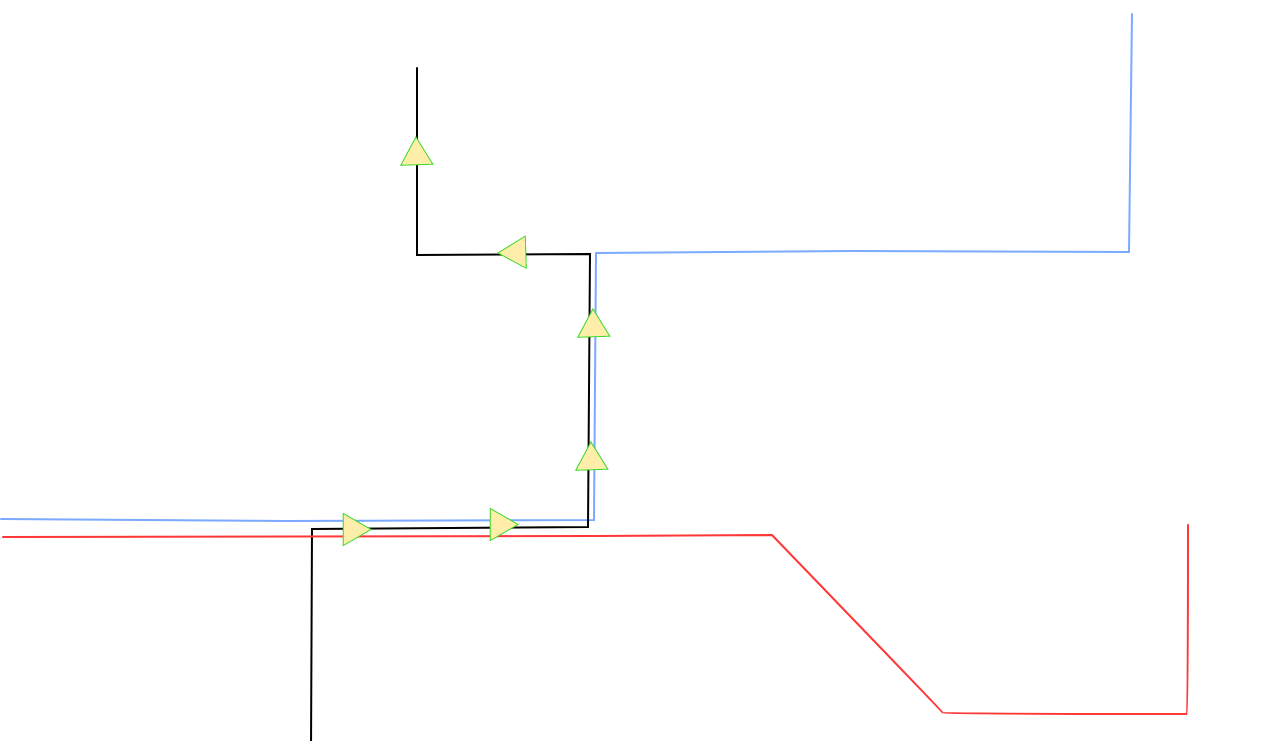
\includegraphics[width=1\textwidth]{images/calculating_route.png}
    \caption{Primjer otkrivanja rute u slučaju preklapanja}\label{fig:calculating_route}
\end{figure}

Primjer otkrivanja moguće rute je prikazan na slici \ref{fig:calculating_route}. Na slici su prikazane 3 različite rute odnosno vozila (crveno, crno, plavo) te lokacije korisnika kao zeleni trokuti. Iako se rute međusobno poklapaju, iz prikazanih lokacija korisnika je očito da korisnik putuje crnom rutom. U slučaju da je poznat samo dio korisnikovih lokacija, primjerice samo prve 3, bi mogli zaključiti da korisnik putuje ili plavom ili crnom rutom no ne bi bilo moguće zaključiti o kojoj se točno ruti radi. U tom slučaju bi trebalo prikupiti još nekoliko korisnikovih lokacija za određivanje točne rute.

Kao što je već bilo spomenuto, potvrda sa strane korisnika u kojem se vozilu nalazi može pozitivno pomoći u otkrivanju točnog vozila no to ne mora uvijek biti slučaj. Naime, može se dogoditi da korisnik slučajno ali i namjerno (maliciozno) odabere krivi broj vozila. Iz toga razloga je bitno na dobivenim podacima prvo provoditi analizu s ciljem utvrđivanja da li korisnik govori istinu. Što se tiče jednostavnih slučajeva kad korisnik kaže da se nalazi u vozilu koje uopće ne prometuje ni blizu korisnikove lokacije, to bi se trebalo i moglo riješiti u samoj klijentskog aplikaciji tako da se za odabir prikažu samo moguća vozila.

S druge strane tu postoji nešto kompleksni slučaj, kada korisnik odabere vozilo u kojem se ne nalazi ali koje putuje tom lokacijom. Ovo se, slično kao i otkrivanje vozila u slučaju bez korisnikove potvrde, može riješiti praćenjem korisnikove lokacije u određenom razdoblju. Drugim riječima, bilo bi potrebno periodički provjeravati da li korisnici govore istinu usporedbom lokacija korisnika te lokacija rute na kojoj korisnik tvrdi da se nalazi.

Najteži slučaj malicioznog korisnika bi bio onaj korisnik koji osim što može govoriti krivi broj vozila, također dijeli krivu lokaciju. Naime, postoje alati ili aplikacije koje omogućuju dijeljenje krive lokacije \engl{location spoofing}. Najčešće se radi o alatima koji zahtijevaju veću razinu pristupa odnosno \emph{root} za Android te \emph{jailbreak} za iOS ili spajanje mobitela na računalo što donekle otežava ovakav napad. Osim nade da će težina izvođenja ovakvog napada natjerati korisnike da ga ne izvode, postoji mogući način otkrivanja koji se temelje na činjenici da lokaciju dijeli više korisnika. Radi se o relativno jednostavnoj provjeri koju je kao i provjeru prethodnog tipa dobro izvoditi periodički. Za svaku grupu korisnika koji se nalaze u istom vozilu se na temelju lokacija korisnika grupe izvodi proces izbacivanja uljeza \engl{outlier}.

\begin{figure}[htb]
    \centering
    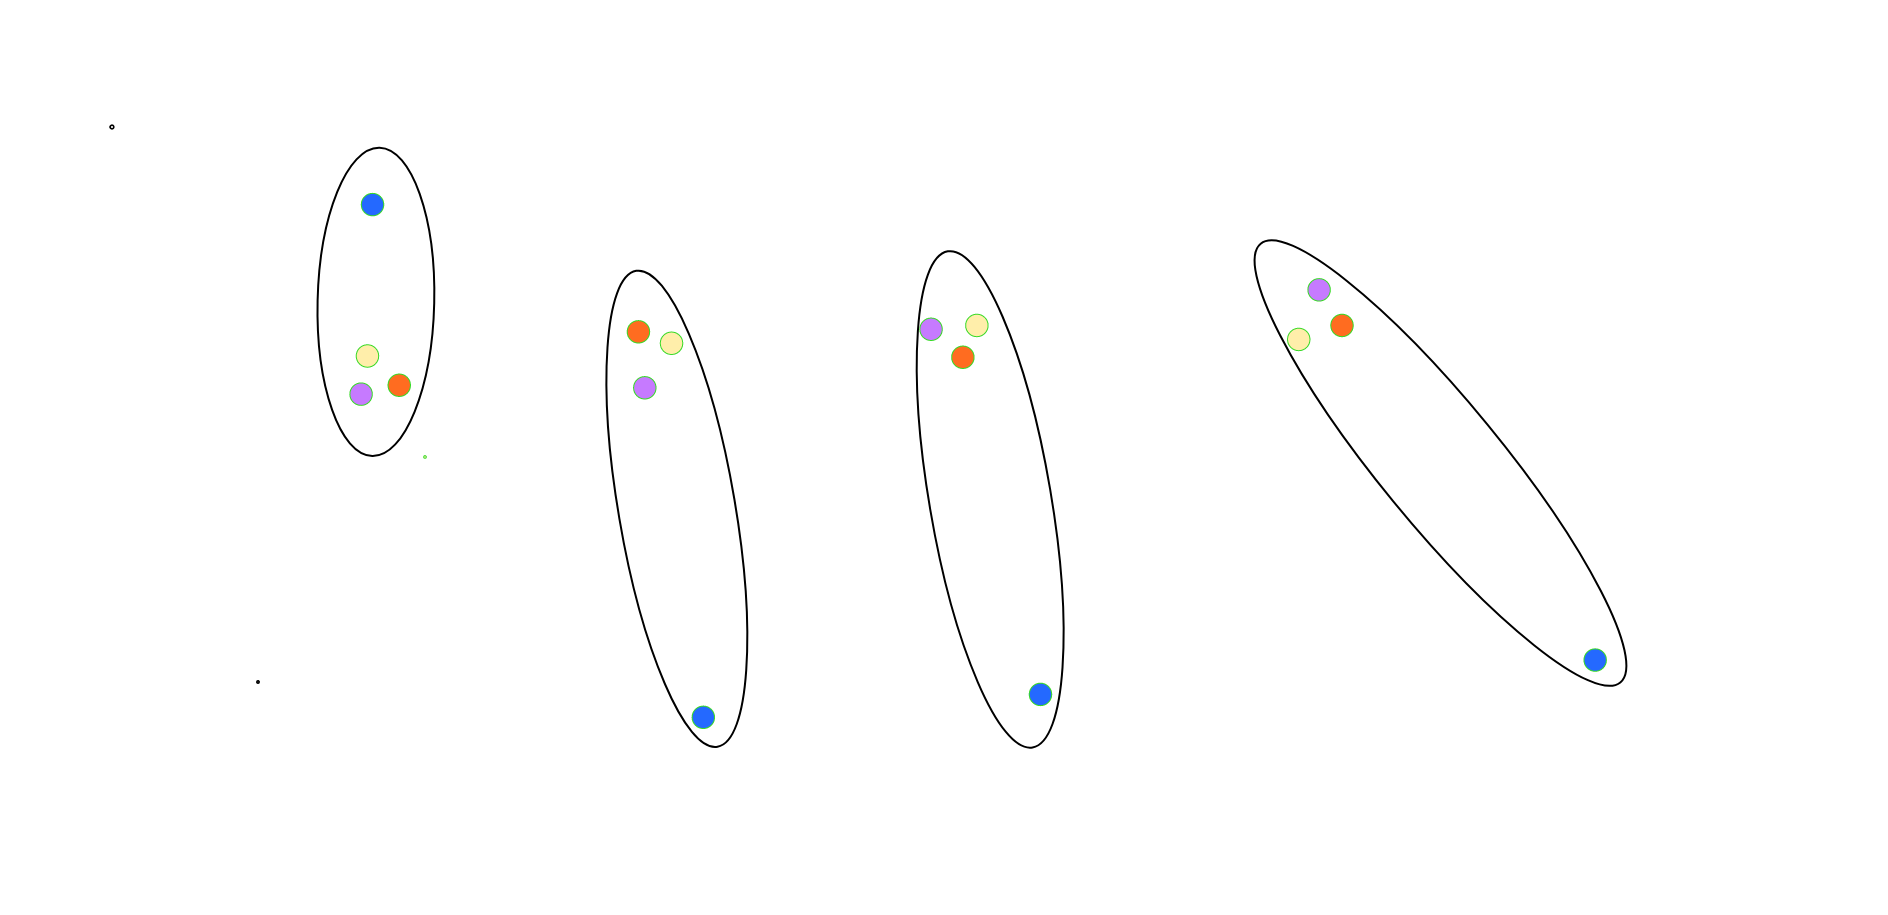
\includegraphics[width=1\textwidth]{images/outlier.png}
    \caption{Primjer \emph{outlier} korisnika}\label{fig:outlier}
\end{figure}

Jednostavan primjer ovakog slučaja je prikazan na prethodnog slici \ref{fig:outlier}. U ovom primjeru imamo 4 korisnika koji su dio iste grupe odnosno koji se voze istim vozilom, ili barem tako tvrde. No lagano se vidi da se lokacije koje plavi korisnik dijeli ne poklapaju s lokacijama drugih korisnika u grupi. Jednostavan algoritam za otkrivanje uljeza bi bio izračunavanje prosječne lokacije odnosno centra te udaljenosti svih članova grupe do centra i zatim odbacivanje onih koji su jako daleko, kao na slici \ref{fig:avg_distances}. Drugi način bi bio izračunavanje međusobnih udaljenosti svih članova grupe te zatim odbacivanje onih koji su jako daleko od svih ostalih, primjer za ovo je na slici \ref{fig:each_distances}.

\begin{figure}
    \centering
    \begin{subfigure}{.5\textwidth}
      \centering
      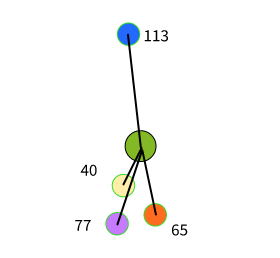
\includegraphics[width=.6\linewidth]{images/outlier_avg_distances.png}
      \caption{Prosječna lokacija}
      \label{fig:avg_distances}
    \end{subfigure}%
    \begin{subfigure}{.5\textwidth}
      \centering
      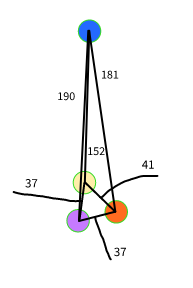
\includegraphics[width=.46\linewidth]{images/outlier_each_distances.png}
      \caption{Meuđusobne udaljenosti}
      \label{fig:each_distances}
    \end{subfigure}
    \caption{Mogući načini odbacivanja \emph{outliera}}
    \label{fig:outliers}
\end{figure}

U prvom primjeru je prosječna lokacija puno bliža trima donjim točkama što se očituje kroz udaljenosti 40,65,77 dok je četvrta točka znatno udaljenija, 113. Sve mjere su izražene u pikselima. U stvarnom svijetu bi algoritam uljeze mogao izbacivati na temelju apsolutnih udaljenosti jer se ipak radi o grupi putnika u istom vozilu, a vozila su ograničenih dimenzija. Osim takvog pristupa, moguće bi bilo i izračunavanje prosječne udaljenosti do centra (u ovom slučaju je to 73.75) te odbacivanje onih čija je relativna udaljenost veća od određene mjere.

U drugom primjeru su prikazane međusobne udaljenosti svih pripadnika grupe. Kao što se lagano može vidjeti, udaljenost plave do ostalih je daleko veća nego udaljenosti preostale 3 međusobno što znači da bi se jednostavno moglo zaključiti koja je točka \emph{outlier}. 


\subsection{Slični radovi i projekti}
Kad su u pitanju radovi koji su se već bavili ovom temom, postoji ih nekoliko:

\begin{itemize}
    \item \textbf{Cooperative Transit Tracking using Smart-phones} (\cite{chicago_cooptransit_tracking})\\
    Rad i istraživanje provedeno na temelju vožnje autobusa i podzemnih vlakova u Chicagu. Pokriva razne probleme vezane uz korištenje grupnog opažanja okoline za praćenje vozila javnog prijevoza kao što su detekcija stanja osobe na temelju akcelerometra, otkrivanja da li se radi o osobnom ili vozilu javnog prijevoza, potrošnju baterije na mobilnim uređajima te druge vezane uz praćenje podzemnih vlakova gdje su signali općenito slabi. Testiranje je bilo napravljeno pomoću simulacije koristeći podatke o stvarnim lokacijama vozila koji su dostupni za Chicago. Rezultati istraživanje pokazuju da čak ako samo 5\% korisnika sudjeluje u ovakvom sustavu se mogu dobiti značajni rezultati kad je u pitanju predviđanje vremena dolazaka.
    
    \item \textbf{Field Trial of Tiramisu: Crowd-Sourcing Bus Arrival Times to Spur Co-Design} \cite{tiramusu} \\
    Rad u kojem je provedeno terensko ispitivanje odnosno istraživanje u stvarnom svijetu sa stvarnim korisnicima. Prikupljanjem povijesti lokacija vozila javnog prijevoza se omogućilo generiranje procjena dolazaka u stvarnom vremenu te osvježavanje statičnih podataka. Ono što je proizašlo iz ovog istraživanje je \emph{Tiramusu} mobilna aplikacija namijenjena za stvarno vremensko predviđanje vremena dolazaka u Pittsburghu. Osim za procjenu vremena dolazaka, aplikacija također ima mogućnost dojave popunjenosti vozila i prijave problema. Nažalost, sudeći prema recenzijama na \emph{Google Play Store}, sustav je prestao raditi 2018. godine.
\end{itemize}



\chapter{Sustav za određivanje lokacija tramvaja na temelju korisničkih podataka}
Ovo poglavlje će se baviti sustavom za otkrivanje lokacija tramvaja. U odnosu na potpoglavlje \ref{section:crowdsensing_system} razlika će biti što će se ovo poglavlje fokusirati na konkretnu implementaciju.

Sustav potreban za ovu aplikaciju bi se mogao realizirati na nekoliko načina odnosno razina kompleksnosti ovisno o načinu na koji bi korisnici koristili aplikaciju --- što je korištenje jednostavnije to bi sustav bio kompleksniji odnosno teži za ostvariti. Zasad razmatrane razine poredane prema kompleksnosti:

\begin{enumerate}
    \item \textbf{Potpuno ručno} - da bi korisnik pokrenuto dijeljenje/slanje lokacije sam pokreće aplikaciju, odabire tramvaja i pokreće uslugu.
    \item \textbf{Automatsko otkrivanje broja tramvaja grupiranjem} - na temelju korisnika koji su trenutno u tramvaju i dijele lokacije. Korisnik i dalje sam pokreće aplikaciju.
    \item \textbf{Automatsko otkrivanje broja tramvaja na temelju povijesti lokacija} - broj tramvaja se otkriva na temelju niza lokacija (povijesti) što znači da nije instantno već treba proći određeno vrijeme. Korisnik i dalje sam pokreće aplikaciju.
    \item \textbf{Otkrivanje ulaska u tramvaj} - aplikacija radi u pozadini i na temelju senzora akcelerometra i GPS-a otkriva kad je korisnik u tramvaju. Ukratko ovo radi na temelju otkrivanja da li je korisnik u vozilu (koristeći akcelerometar) te ako je da li je u vozilu tramvaja (koristeći GPS) provjerava da li je ruta kojom se korisnik kreće slična ruti za tramvaje koji voze u tom području. Kad se otkrije da je korisnik u tramvaju šalje se notifikacija koja pita korisnika da li je željan dijeliti lokaciju.
    \item \textbf{Potpuno automatski} - prethodna razina ali uz opciju da korisnik uključuje i isključuje uslugu dijeljenja po potrebi.
\end{enumerate}


\section{Opis sustava}
Razine koje su implementirane u sustavu simulacije za rad su prve 3, iako s obzirom na to da se radi o simulaciji razine 4 i 5 ne bi niti mogle biti implantirane, barem ne na jednostavan i realan način, jer zahtijevaju senzore poput akcelerometra.

Prije nego što se krene opisivati rad sustava, bitno je obratiti pozornost na kako su glavne komponente sustava spremljene. U nastavku slijedi pregled glavnih i pomoćnih struktura podataka.

\subsection{Strukture podataka}
Što se tiče spremanja podataka potrebnih za rad sustava, korišteno je sljedeće:
\begin{itemize}
    \item lokacija s vremenom (\textbf{vremenska lokacija}) - geografske koordinate uz vrijeme bilježenja. Vrijeme je predstavljeno kao cijeli broj koji označuje proteklo vrijeme od početka rada simulacije;
    \item \textbf{tram} - predstavlja predviđeni tramvaj na temelju lokacija putnika. Označen kao [broj tramvaja (rute), smjer (0 ili 1), indeks (jer može postojati više tramvaja istog broja i smjera)];
    \item \textbf{passenger} - putnik, predstavljen kao objekt iz simulacije. Preko javnih metoda; omogućuje dobivanje lokacije te broja tramvaja. Ovisno o kakvom se putniku radi, podaci mogu biti neistiniti (maliciozni putnik) ili nepotpuni (neutralni putnik);
    \item \textbf{passenger\_location\_deque} - mapa [\emph{putnik} -> ograničeni red prethodnih vremenskih lokacija] - koristi se za pamćenje povijesti lokacija putnika;
    \item \textbf{passenger\_first\_location} - mapa [\emph{putnik} -> prva prijavljena vremenska lokacija] - pomoćna struktura korištena za otkrivanje putnikove rute ili provjeru istinitosti;
    \item \textbf{passengers\_in\_trams} - mapa [\emph{tramvaj} -> set putnika u tramvaju] - služi za grupiranje putnika u grupe koje predstavljaju tramvaje;
    \item \textbf{passenger\_tram\_map} - mapa [\emph{putnik} -> \emph{tramvaj}] - pomoćna struktura korištena za ubrzanje određenih akcija poput uklanjanja putnika sustava jer bi se u suprotnom trebalo prolaziti po svim grupama dok se ne nađe traženi putnik;
    \item \textbf{tram\_location\_deque} - mapa [\emph{tramvaj} -> ograničeni red prethodnih vremenskih lokacija] - koristi se za pamćenje povijesti lokacija tramvaja;
    \item \textbf{tram\_indexes} - mapa [\emph{(broj tramvaja, smjer)} -> set indeksa] - koristi se za praćenje različitih tramvaja istog broja i smjera;
    \item \textbf{passenger\_update\_scheduler} - mapa [\emph{vremenski period} -> set putnika] - koristi se za raspoređivanje periodičkog osvježavanja lokacija putnika;
    \item \textbf{passenger\_scheduler\_map} - mapa [\emph{putnik} -> \emph{vremenski period}] - isto kao \emph{passenger\_tram\_map} ali za raspoređivač osvježavanja lokacija.
\end{itemize}

\subsection{Korišteni alati i pomoćne metode}
Od alata i programskih biblioteka je korišteno sljedeće:
\begin{itemize}
    \item Python 3.9,
    \item Numpy,
    \item Sklearn
\end{itemize}

U ovom dijelu će biti ukratko opisane neke od pomoćnih metoda korištenih u implementaciji.

Prva od metoda je ona za računanje sličnosti 2 niza lokacija. Osim ta 2 niza, kao argument metoda također prima i radijus u metrima. Taj radijus označuje udaljenost u kojoj se obavlja pretraga. Naime, za svaku točku (par koordinata) jednog od nizova lokacija, se uspoređuju točke drugog niza te se vraća broj točaka unutar radijusa. Nakon toga, se kao finalni rezultat vraća omjer broja točaka za koje je u radijusu pronađena susjedna točka te ukupnog broja točaka. Za olakšavanje implementacije je korištena već spomenuta programska knjižnica \texttt{sklearn}, točnije \texttt{BallTree} struktura podataka kojoj je svrha ubrzati prostorne pretrage. Za računanje udaljenosti se koristi \emph{haversine} mjera jer je pogodna za računanje geografskih udaljenosti.

\begin{figure}[htb]
    \centering
    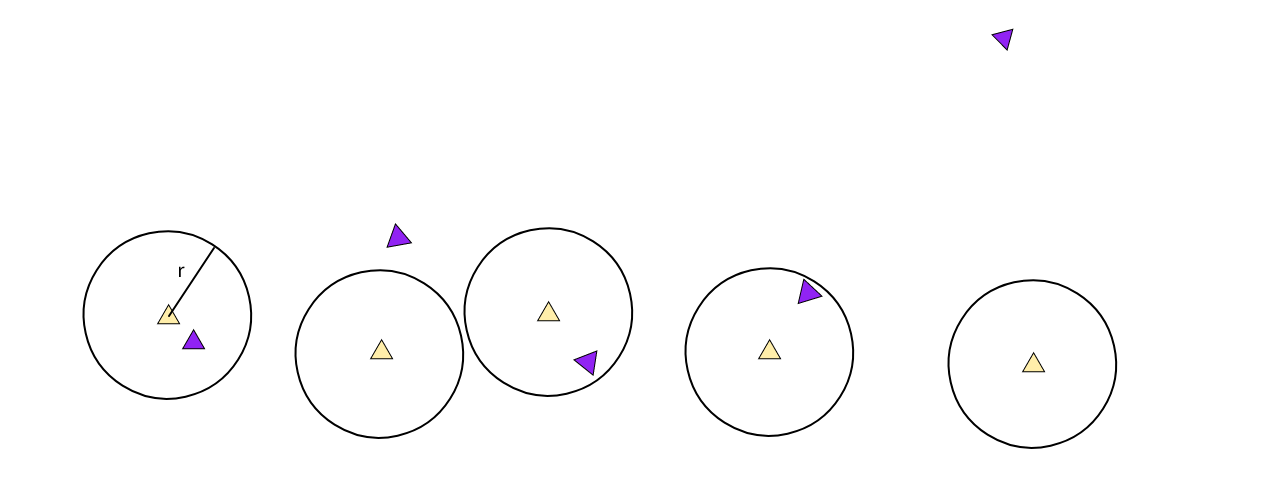
\includegraphics[width=1\textwidth]{images/location_history.png}
    \caption{Usporedba sličnosti niza lokacija}\label{fig:location_history_comparison}
\end{figure}

Kao što se može vidjeti na slici \ref{fig:location_history_comparison}, usporedbom 2 niza točaka možemo zaključiti kako je sličnost 0.6 odnosno 60\%, jer 3 od ukupno 5 točaka niza u određenom radijusu ima susjeda iz drugog niza. Pseudokod slijedi u nastavku:

\begin{lstlisting}[caption={Usporedba povijesti lokacija},captionpos=b,label={kod:location_history_comparison}]
    def get_route_similarity(points1, points2, radius = 125):
        points2 = np.deg2rad(points2)
        bt = BallTree(np.deg2rad(points1), metric='haversine')
        in_radius = bt.query_radius(points2, radius, count_only=True)
        return np.count_nonzero(in_radius) / len(in_radius)

\end{lstlisting}

Sljedeća pomoćna metoda se koristi za brzo određivanje mogućih tramvajskih ruti na temelju prve i zadnje točke u nizu lokacija. Ovo prvenstveno služi kao prva razina filtriranja u određivanju one rute koja najbolje odgovara nizu točaka, o čemu će više riječi biti kasnije. Ukratko, za prvu i zadnju točku se dobivaju 3 najbliže stanice te skupovi tramvaja koji putuju njima te se kao mogući tramvaji vraća unija tih skupova. Osim uspoređivanja više točaka, znači ne samo prve i zadnje, moguće poboljšanje ove metode bi moglo biti vraćanje samo onih tramvajskih linija koje putuju i prvom i zadnjom odnosno presjek za razliku od unije. Problem s ovakvim pristupom bi bio nepoželjno odbacivanje linija.

\begin{lstlisting}[caption={Određivanje mogućih tramvajskih ruta},captionpos=b,label={kod:possible_tram_routes}]
    def get_possible_tram_routes(self, points):
        possible_tram_routes = set()
        closest_stops1 = get_closest_stops(points[0], n=3, radius = 125)
        closest_stops2 = get_closest_stops(points[-1], n=3, radius = 125)
        stops = closest_stops1 + closest_stops2
        for stop in stops
            possible_tram_routes.update(get_routes_for_stop(stop))
        return possible_tram_routes

\end{lstlisting}

Prethodne metode su bitne za sljedeću jer se radi o traženju najsličnije tramvajske rute za određeni niz lokacija. Ovo se koristi prilikom grupiranja korisnika. Prvo se pomoću \texttt{get\_possible\_tram\_routes} dobiju moguće tramvajske rute koje se zatim uspoređuju sa zadanim nizom lokacija koristeći metodu \texttt{get\_route\_similarity}. Na kraju se vraća ona najsličnija.

\begin{lstlisting}[caption={Traženje najbliže tramvajske rute},captionpos=b,label={kod:closest_tram_route}]
    def find_closest_tram_route(points, radius: int = 100):
        possible_tram_routes = get_possible_tram_routes(points)

        (closest_route, similarity) = find_closest_route(points, possible_tram_routes)
        return (closest_route, similarity)

\end{lstlisting}


\subsection{Prijavljivanje putnika u sustav}
Prilikom ulaska putnika u vozilo i početka dijeljenja lokacije se ovisno o tipu putnika događaju sljedeće stvari, ako se radi o putniku za kojeg nije poznat broj i smjer tramvaja, putnik ulazi u raspoređivač periodičkog osvježavanja lokacija. Razlog za uvođenje raspoređivača je raspoređivanje putnika u nekoliko skupina tako da se lokacije putnika ne osvježavaju sve odjednom (što bi moglo negativno utjecati na performanse). Vremenska skupina se određuje prema sljedećoj formuli:
\begin{equation} \label{formula:schedule_time}
    \ceil*{(time\;\%\;(10*n))\:/\:10}
\end{equation}

gdje \emph{n} predstavlja broj skupina. Primjerice za \emph{n=3} uz trenutno vrijeme 25 će odabrana skupina biti \emph{2} dok će za vrijeme 31 biti odabrana skupina \emph{0}.

S druge strane, ako je za putnika poznat broj tramvaja i smjer, putnik se odmah grupira. Postupak grupiranja slijedi u nastavku.


\subsection{Grupiranje putnika}
Ako se radi o putniku čiji je broj tramvaja i smjer poznat, grupiranje se odvija na sljedeći način:

\begin{lstlisting}[caption={Grupiranje putnika s poznatim podacima},captionpos=b,label={kod:group_positive}]
    if check_malicious_by_closest_stop(passenger):
        put_passenger_into_scheduler(passenger)
    let group
    if len(groups[passenger.tram]) == 0:
        group = (passenger.tram, 0)
    elif ((best_group = check_if_fits_existing_groups(passenger)) is not None):
        group = best_group
    else:
        group = get_new_group(passenger.tram)
    add_passenger_to_group(group, passenger)

\end{lstlisting}

Kao što se vidi iz pseudokoda \ref{kod:group_positive}, prvo se na temelju lokacije putnika provjerava da li putnik uopće može biti u tom tramvaju. Radi se o jednostavnoj provjeri gdje se uspoređuju svi mogući tramvaji u blizini s tramvajem u kojem se putnik nalazi ili barem tvrdi. Primjerice, ako se putnik nalazi na Vukovarskoj ulici kod križanja s Heinzlovom gdje prometuju tramvaji 2,3,13 znamo da se ne može nalaziti u tramvaju 1.
Nakon toga slijedi provjera postojećih grupa odnosno određivanje grupe u koju će se putnika staviti. Ako u sustavu nema grupa za taj tramvaj, stvara se nova s indeksom 0.\\
Ako postoji grupa koja odgovara, što znači da je zadnja lokacija grupe blizu lokacije putnika, to će biti odabrana grupa.
U suprotnome, stvara se nova grupa s prvim sljedećim indeksom.
Kad se odredi prava grupa, putnika se stavlja u nju.


Drugi slučaj je kad se za putnika ne zna broj tramvaja i smjer (ili je sustav detektirao da se radi o neistinitom tramvaju):
\begin{lstlisting}[caption={Grupiranje putnika s nepoznatim podacima},captionpos=b,label={kod:group_neutral}]
    let group
    previous_locations = passenger_location_deque[passenger]
    (best_group, certainty) = find_best_group_based_on_previous_locations(previous_locations)
    if certainty > 0.9:
        group = best_group
    else:
        (closest_tram_route, similarity) = find_closest_tram_route(previous_locations)
        if similarity >= 0.3:
            group = get_new_group(closest_tram_route)
    if group is not None:
        add_passenger_to_group(group, passenger)
        remove_passeger_from_schedule(passenger)

\end{lstlisting}
Za razliku od prethodnog algoritma, ovdje se uspoređuje povijest lokacija putnika s povijestima lokacija trenutno aktivnih grupa. Ako se pronađe adekvatna grupa, putnika se stavlja u nju. Ako nema aktivnih grupa koje odgovaraju, za putnika se pokušava odrediti u kojem se tramvaju nalazi. U slučaju da je podudaranje dovoljno značajno, putnika se stavlja u novu grupu s pripadajućim indeksom. U oba slučaja se putnika briše iz raspoređivača.

Ako nijedno od prethodna 2 slučaja ne prođe što uglavnom znači da u sustavu nema dovoljno informacija o putniku, putnik i dalje ostaje u raspoređivaču.

\subsection{Pamćenje lokacija putnika i tramvaja}
Raspoređivač osvježavanja lokacija putnika je jednostavna komponenta odnosno metoda koja svakih 10 sekundi provjerava trenutno aktivno vrijeme prema formuli \ref{formula:schedule_time} te za sve putnike u tom skupini osvježi lokaciju odnosno doda novu u red lokacija za tog putnika. Uz to, za svakog putnika poziva metodu grupiranja.

Slično se radi i osvježavanje lokacija grupi ili tramvaja. Bitna razlika je što se tramvaji sastoje od više putnika pa je dobivanje lokacije nešto drugačije. Naime zbog preciznosti se uzimaju lokacije više od jednog putnika te se računa prosječna lokacija. Broj putnika čije se lokacije uzimaju u obzir je maksimalno pola putnika te se putnici odabiru na nasumičan način.

\section{Potencijalni problemi i moguća rješenja}

\subsection{Izlazak iz tramvaja}

Ono što je bitno napomenuti jest problem kako s korisničke strane realizirati izlazak iz tramvaja odnosno prekid usluge dijeljenja lokacije. Naime tu postoji nekoliko situacija koje bi mogle biti vrlo komplicirane. Pri izlasku iz tramvaja se može dogoditi da korisnik ne zaustavi uslugu dijeljenja lokacije. To se može dogoditi slučajno (korisnik zaboravi ugasiti uslugu) ili namjerno, ne nužno i ne maliciozno (ako zna da će uskoro ući u drugi tramvaj). U tom slučaju postoje 2 (glavna) tijeka događaja. Prvi je da se korisnik pješice udalji od stanice na kojoj je izašao, drugi je da ostane stajati na toj stanici. U slučaju da ostane na stanici mogli bi pretpostaviti da čeka neki od idućih tramvaja ili da čeka nekoga na toj stanici. S druge strane, kompliciraniji tijek događaja je kad se korisnik udalji od stanice. Razlozi za to mogli biti:
\begin{itemize}
    \item treba presjesti na drugi tramvaj koji vozi stanicom koja je u blizini no treba pješice doći do nje;
    \item blizu je odredišta na kojem planira biti stacionaran (posao, kuća);
    \item blizu je odredišta na kojem ne planira biti stacionaran (planira ući u automobil, bus...)
\end{itemize}

Što se tiče mogućih rješenja za problem izlazaka, ako se pretpostavi da je na neki način moguće detektirati da korisnik više nije u tramvaju, tu postoje 2 moguća skupa rješenja:
\begin{itemize}
    \item ono jednostavnije ali ne "user friendly" -- nakon detekcije usluga se sama zaustavi. Ovo može biti problem u slučaju da ju korisnik namjerno nije isključio jer je znao da će uskoro ući u sljedeći tramvaj;
    \item kompliciranije -- uključuje praćenje akcija korisnika nakon izlaska s ciljem otkrivanja hoće li korisnik nastaviti putovanje nekim drugim tramvajem.

\end{itemize}


\subsection{Pogreške u radu sustava}
Smišljeni sustav nije savršen što je razumljivo jer podaci s kojima se radi također nisu savršeni. Osim već spomenutih malicioznih korisnika, neke od pogrešaka koje se mogu dogoditi su krivo označene grupe odnosno tramvaji ili krivo grupirani korisnici. Radi se o sličnim pogreškama pa samim time i sličnim rješenjima.
Što se tiče krivo označenih korisnika, uzrok može biti ili napad na sustav (maliciozni korisnik) ili jednostavno pogreška uzrokovana nedostatkom informacija. Rješenje za otkrivanje \emph{outlier} korisnika je relativno jednostavno. Kao što je već bilo pokazano u primjeru \ref{fig:outliers} u prethodnom poglavlju, 2 moguća načina su računanje prosječne lokacije grupe te računanje međusobnih udaljenosti članova grupe. U nastavku slijede pseudokodovi tih metoda:

\begin{lstlisting}[caption={Otkrivanje \emph{outliera} - prosječna lokacija},captionpos=b,label={kod:outlier_average}]
    def detect_outlier_by_avg(points, max_distance=40):
        center = average_point(points)
        distances = [calculate_distance_haversine(center, p) for p in points]
        avg_distance = calculate_average(distance)
        distance_diffs = [d - avg_distance for d in distances]
        possible_outlier_index = index_of_max(distance_diffs)

        if distance_diffs[possible_outlier_index] > max_distance: return possible_outlier_index
        else return None

\end{lstlisting}

Prva metoda koja radi na temelju centra grupe prvo računa prosječnu točku, zatim udaljenosti svih točaka do centra i prosječnu udaljenost. Naposljetku, računa razlike između prosječne udaljenosti i svih udaljenosti te kao rezultat vraća indeks one točke s maksimalnom razlikom ali samo ako je ta razlika veća od postavljenog uvjeta \emph{max\_distance}.

\begin{lstlisting}[caption={Otkrivanje \emph{outliera} - međusobne udaljenosti},captionpos=b,label={kod:outlier_each}]
    def detect_outlier_by_distances(points, max_distance=40):
        avg_distances = [0] * len(points)
        for i in range(len(points)):
            pi = points[i]
            for j in range(i+1, len(points)):
                pj = points[j]
                distance = calculate_distance_haversine(pi,pj) / (len(points) - 1)
                avg_distances[i] += distance
                avg_distances[j] += distance
        avg_avg = calculate_average(avg_distances)
        distance_diffs = [(i, d - avg_avg) for i,d in enumerate(avg_distances) if (d - avg_avg) > max_distance]
        if len(distance_diffs) == 0: return None
        possible_outlier = max(distance_diffs, key = lambda p : p[1])

        return possible_outlier[0]

\end{lstlisting}
Prvi dio ove metode za svaku točku računa prosječnu udaljenost do ostalih točaka tako da u listu koja je inicijalizirana nulama (\emph{avg\_distances}), na pravi indeks dodaje izračunatu udaljenost za par točaka podijeljenu sa (\emph{broj\_točaka - 1}). Drugi dio metode je gotovo isti kao prethodna metoda \ref{kod:outlier_each}. Razlika je što se ovaj put računa prosjek prosječnih udaljenosti te se kao rezultat vraća indeks one koja ima najveću razliku uz to da je uvjet \emph{max\_distance} zadovoljen.

Neovisno koja metoda bude odabrana za ovu funkcionalnost, za optimalan rad bi se trebala pozivati periodički. Putnici za koje se bude smatralo da su uljezi mogu biti ili izbačeni iz sustava ili vraćeni u sustav kao neutralni.\\


Sljedeći problem su krivo označene grupe i grupe koje ne bi trebale postojati. Situacija u kojoj bi moglo doći do krivo označene grupe je prikazana na slici \ref{fig:calculating_route} iz prethodnog poglavlja. Naime, u slučaju da je poznat samo dio prikazanih lokacija korisnika, sustav bi mogao odrediti da se korisnik nalazi u ruti označenoj s plavom bojom što nije istina. Ovo bi zahtijevalo periodičku usporedbu povijesti lokacija grupe s nizom lokacija rute pripisane toj grupi. 

Drugi problem su nepostojeće grupe. Mogući uzrok bi mogao biti prethodni problem. Primjerice, ako u krivo označeni tramvaj uđe korisnik koji tvrdi da se nalazi u drugom tramvaju, sustav će tog novog korisnika grupirati odvojeno, kao novu grupu. Nakon nekog vremena, kad se krivo označeni tramvaj prepravi, u sustavu bi postojale 2 grupe koje imaju istu oznaku (broj tramvaja, smjer) no različiti indeks. Njihove povijesti lokacija bi također bile jako slične. Rješenje je prikazano sljedećim pseudokodom:

\begin{lstlisting}[caption={Provjera nepostojećih grupa},captionpos=b,label={kod:group_check}]
    def _group_checker():
        for num_dir,num_dir_index_list in tram_indexes_map.items():
            if len(num_dir_index_list) <= 1: continue
            to_skip_and_delete = set()
            seen = set()
            for tram1 in (num_dir_index_list - to_skip_and_delete - seen):
                seen.add(tram1)
                locations1 = tram_location_deque[tram1]
                for tram2 in (num_dir_index_list - to_skip_and_delete - seen):
                    locations2 = tram_location_deque[tram2]
                    similarity = stopRouteComparator.get_route_similarity(locations1, locations2, 60)
                    if similarity > 0.85:
                        transfer_passengers(from_tram=tram2, to_tram=tram1)
                        to_skip_and_delete.add(tram2)
            for tram in to_skip_and_delete:
                del passengers_in_trams[tram]
                del tram_location_deque[tram]
                tram_indexes_map[num_dir].remove(tram)

\end{lstlisting}

Ukratko, za svaku liniju (broj tramvaja i smjer) za koju u sustavu postoji više trenutno aktivnih tramvaja, se uspoređuju povijesti lokacija svih tih aktivnih tramvaja. U slučaju da se nađe par čije su povijesti lokacija dovoljno slične, te grupe se spajaju tako da se svi putnici iz druge premjeste u prvu.


\subsection{Komunikacija}
Kako je implementacija sustava napravljena kroz simulaciju, postavlja se pitanje koji je najbolji način da se komunikacija između korisnika i sustava napravi. S obzirom na to da sam sustav zadužen za upravljanje pamćenja lokacija korisnika, ta komunikacija ne bi mogla biti jednosmjerna od korisnika prema sustavu. Moguće rješenje je korištenje dvosmjerne komunikacije kao što je \emph{TCP socket} gdje sustav korisniku šalje zahtjeve za lokaciju i slično.

\subsection{Skalabilnost}
Kako sam rad ne sadrži pravu implementaciju sustava već samo simulaciju, jedan od bitnih aspekata svakog sustava koji nije mogao biti pravilno testiran je skalabilnost.
Ovo bi mogao biti problem ovisno o odazivu broja korisnika koji bi bili voljni dijeliti lokaciju.
Naime, broj korisnika može biti problem kad je premali jer predikcije lokacija ne bi bile potpune ili bi bile nedovoljno točne. S druge strane, preveliki broj korisnika može uzrokovati usporeni rad sustava ili čak netočne informacije o lokacijama tramvaja jer sustav nije prilagođen za rad s toliko korisnika u isto vrijeme. 
Neki od mogućih rješenja za ovakve probleme bi bili kontrola broja korisnika, kako globalno tako i po regiji grada ili tramvajskoj liniji.




\chapter{Analiza GTFS (General Transit Feed Specification) datoteka}
\section{O GTFS datotekama ZET-a}
Ove datoteke definiraju i opisuju standardizirani format podataka za javni prijevoz.\\
Radi se o .zip datoteci koja u sebi sadrži nekolicinu .txt datoteka u csv formatu. U slučaju Zagreba odnosno ZET-a dostupne su sljedeće datoteke:\\
\begin{itemize}
    \item \emph{agency.txt},
    \item \emph{calendar.txt},
    \item \emph{calendar\_dates.txt},
    \item \emph{feed\_info.txt},
    \item \emph{routes.txt},
    \item \emph{stop\_times.txt},
    \item \emph{stops.txt},
    \item \emph{trips.txt}
\end{itemize}

\emph{agency.txt} i \emph{feed\_info.txt} samo sadrže podatke o agenciji (primjerice poveznicu na stranicu, puno ime...) te podatke poput vremena važenja ovih datoteka i slično. Uglavnom radi se o datotekama koje nije potrebno analizirati. Potpuno nebitna datoteka je \emph{calender.txt}. Prema pravilima GTFS-a ova datoteka bi trebala sadržavati podatke o vrstama usluge koje se redovno ponavljaju. Vrsta usluge može biti radni dan, vikend, praznik, itd. U ovom slučaju ZET nije definirao takva ponavljanja pa ovu datoteku također možemo ignorirati u analizi. Na svu sreću, ZET je zato pružio datoteku \emph{calendar\_dates.txt} koja definira vrstu usluge za svaki datum u određenom razdoblju. Postoji 9 različitih vrsta usluge koje je ZET definirao, \emph{0\_1} se koristi za radne dane, \emph{0\_2} za subote, \emph{0\_3} za nedjelje. Ostali se koriste za razne blagdane (nije baš potpuno jasno). \\
\emph{stops.txt} kako samo ime govori predstavlja datoteku koja sadrži informacije o stanicama. Te informacije moraju sadržavati jedinstveni identifikator stanice, naziv stanice, geografsku širinu i dužinu dok također mogu imati podatke poput opisa stanice, id zone, poveznicu (url) stanice, vrstu stanice i roditeljsku \engl {parent} stanicu. ZET je ustupio samo potrebne. Sljedeća bitna datoteka je \emph{routes.txt} koja sadrži opise svih linija. Od bitnih informacija tu su id linije, naziv kao \emph{polazište} - \emph{dolazište} te vrsta linije (ZET koristi 0 za tramvaje te 3 za buseve). Druga po veličini je datoteka \emph{trips.txt} koja sadrži sve vožnje u nekom razdoblju. Vožnja je definirana pomoću šifre linije (broj vozila), vrste usluge, nazivom krajnje stanice, smjerom (0 ili 1) te identifikatorom bloka za koji mi nije jasno što točno predstavlja. Za razdoblje od 8.2.2021. do 20.6.2021. ova datoteka sadrži skoro 94000 vožnji. Posljednja i najveća, a vjerojatno i najbitnija datoteka jest \emph{stop\_times.txt}. Radi se o datoteci koja definira vremena dolazaka na stanice za sve stanice svake vožnje. Svaka linija sadrži id vožnje (kao što je definirano u \emph{trips.txt}), vrijeme polaska i dolaska (koji su iz nekog zanimljivog razloga jednaki u slučaju ZET-a), id stanice, redni broj stanice u vožnji te naziv krajnje stanice. Ono što je posebice zanimljivo je da je vrijeme dolaska/polaska ponekad definirano u formatu 0-24, a ponekad prelazi 24 (ide do 29)

\section{Analiza i dobivanje korisnih informacija}
Svrha analize GTFS datoteka uključuje sljedeće:
\begin{itemize}
    \item odvajanje podataka za buseve i tramvaje;
    \item filtriranje nepotrebnih i nepotpunih podataka --- neki stupci su ili jednaki za sve ili potpuno nebitni za rad aplikacije;
    \item dobivanje vremena putovanja između stanica --- uključujući susjedne i nesusjedne stanice;
    \item dobivanje udaljenosti između stanica --- iako se iz podataka ZET-a može izvući samo zračna udaljenost to bi i dalje moglo biti korisno u predviđanju vremena dolaska tramvaja;
    \item dobivanje popisa tramvaja/ruti koje putuje određenom stanicom
\end{itemize}

Odvajanje podataka je potrebno jer je barem za prvu verziju aplikacije namijenjeno da bude samo za tramvajski prijevoz. Razlog za ovo je smanjenje kompleksnosti --- iako su podaci identični, buseva ima puno više, a i za razliku od tramvaja koji voze po pruzi, busevi voze cestom što znači da može doći do većih promjena u ruti što bi moglo otežati otkrivanje lokacije/trenutne rute.\\
Što se tiče filtriranja nebitnih podataka za primjer bi se mogla uzeti datoteka \emph{calendar\_dates.txt}. Ona osim već spomenutih podataka sadrži stupac \emph{exception\_type} koji je identičan za sve datume i pridružene vrste usluga. Osim toga, u nekim datotekama postoje stupci koji sadrže prazne podatke.\\
Vrijeme putovanja između stanica se dobilo analizom datoteke \emph{stop\_times.txt} pomoću razlika u vremenima dolazaka na stanicu (izraženo u formatu HH:MM:SS). Osim vremena putovanja između susjednih stanica, također je i bitno vrijeme putovanja između nesusjednih odnosno onih parova stanica koje su odvojene ili između kojih postoji jedna ili više stanica. Ovo se može izraziti kao zbroj vremena putovanja svih susjednih stanica na istoj ruti. Ono što je bitno napomenuti jest da vremena putovanja nisu bila jednaka za sve tramvaje (što možda je očekivano s obzirom na to da postoje nekoliko vrsta tramvaja, starih i novijih) no također nisu bila jednaka za isti tramvaj (isti broj/id). Na svu sreću razlike u vremenima nisu značajne (svakodnevni promet uključuje semafore i druge stvari koje mogu jako utjecati na vremena putovanja između stanica). No ipak postoje čudni podaci poput toga da vrijeme putovanja između stanica \emph{Prisavlje} i \emph{Vjesnik} može iznositi (u sekundama) [150, 180, 210, 240], a ponekad i [90, 94]. Ovo nije isto za svaki broj tramvaja ili svaku vrstu usluge (radni dan, vikend...). Naravno jedna od mogućih funkcionalnosti aplikacije jest bilježenje stvarnih vremena putovanja između stanica (ovisno o tramvaju, dobu dana, vrsti dana...).\\
Zračna udaljenost između stanica bi mogla biti korisna pri predviđanju brzine putovanja tramvaja između tih stanica tako da se brzina računa kao omjer udaljenosti i vremena putovanja. Ovo znači da se radi o aproksimaciji jer u stvarnosti nisu svi putevi između stanica ravne linije.


\chapter{Simulacija}
Testiranje ovakvog sustava u stvarnom svijetu bi moglo biti jako zahtjevno zbog veliki broj korisnika/testera koji bi bili potrebni, barem što se tiče testiranja rada samog algoritma. Zato je odlučeno da će se testiranje prvo provesti koristeći simulaciju uz sljedeće napomene:

\begin{itemize}
    \item samo dnevni tramvaji;
    \item korišteni su samo podaci za "normalne" dane odnosno tip usluge "0\_1";
    \item nisu korištena stvarna vremena polazaka nego su na početku simulacije određena nasumična vremena stvaranja tramvaja. Stvaranje tramvaja se događa samo na početku simulacije;
    \item tramvaji nikad ne staju s radom. Kada stignu na zadnju stanicu u ruti se samo okrenu i to ponavljaju cijelo vrijeme;
    \item korisnici se stvaraju na nasumičnoj stanici s nasumičnim ciljem (broj tramvaja i stanicom); 
    \item prilikom dolaska na cilj, korisnici nestaju iz simulacije;
    \item tipovi korisnika: neutralan (ne dijeli broj tramvaja i smjer nego samo lokaciju), dobar (koristi aplikaciju na ispravan način -- kad uđe u tramvaj upiše točan broj i smjer tramvaja) te maliciozan (upisuje krivi broj tramvaja);
    \item tramvaji putuju različitim brzinama;
    \item tramvaji se ne mogu preteći;
    \item potrebno je simulirati zastoje koji nisu čekanje na stanici (semafori). Lokacije zastoja ne moraju imati smisla (odnosno biti na raskrižju);
    \item put između stanica je predočen kao ravna linija (zbog jednostavnosti);
    \item lokacije koje korisnici šalju su nasumično pomaknute od stvarnih -- zbog nepreciznosti GPS-a u stvarnom svijetu;
    \item sustav za otkrivanje lokacija tramvaja prima samo lokacije i opcionalno broj tramvaja korisnika. Ne zna za stvarne lokacije.
\end{itemize}

\subsection{Korišteni alati}
U ovom dijelu će biti nabrojani alati koji su korišteni u simulaciji te na koji način. Uglavnom se odnosi na programske jezike i programske knjižnice. Radi se o sljedećem:
\begin{itemize}
    \item \textbf{Python 3} - korišten za izgradnju glavnog (\emph{backend}) dijela simulacije;
    \item \textbf{Fastapi, Asyncio} - programske knjižnice, korištene za omogućavanje WebSocket komunikacije s vizualnim ((\emph{frontend}) dijelom simulacije;
    \item \textbf{HTML, JavaScript} - korišteni za prikazivanje odnosno vizualiziranje simulacije. Za prikaz karte je korišten Google Maps JS (Maps JavaScript API)
\end{itemize}

\section{Način rada i dijelovi simulacije}
U ovom dijelu će biti riječ o načinu rada (glavnoj ideji) simulacije te komponentama koje čine simulaciju. Sve komponente će biti detaljnije opisanu u pripadajućim potpoglavljima.
Ukratko, simulacija radi u koracima od 1 sekunde. U svakom koraku glavna komponenta simulacije upravlja svim ostalim dijelovima govoreći im da naprave sljedeći korak te vrate pripadne rezultate odnosno njihovo stanje. Uključujući glavnu komponente su sljedeće:
\begin{itemize}
    \item komponenta koja komunicira sa \emph{frontend} dijelom,
    \item glavna komponenta koja upravlja s ostalima,
    \item komponenta koja upravlja tramvajima, \emph{TramManager},
    \item komponenta koja zastojima i redoslijedom na pruzi, \emph{QueueManager},
    \item komponenta koja upravlja stanicama, \emph{StopManager},
    \item komponenta koja upravlja putnicima, \emph{PassengerManager},
    \item komponenta koja bilježi bitne događaje, \emph{Logger},
    \item komponenta za vizualni prikaz simulacije. S obzirom na to da se radi o jednostavnoj HTML datoteci s pripadajućom skriptom (JavaScript) ova komponenta je odvojena od ostatka.
\end{itemize}


Bitno je napomenuti kako komponente međusobno komuniciraju, primjerice tramvaji imaju referencu na \emph{StopManager} preko koje dojavljuju stanicama da su stigli na njih pa zatim pojedina stanica preko reference na \emph{PassengerManager} može dojaviti određenom putniku da je određeni tramvaj na određenoj stanici.


U nastavku slijede detaljniji opisi svih komponenti.

\subsection{Vizualna komponenta}
Sastoji se od HTML-a koji definira vizualne elemente i Javascript koda koji je zadužen za definiranje logike interaktivnih elemenata (gumbiju, text inputa) te primanje podataka od \emph{backenda}. Glavna svrha ove komponente je za vizualiziranje same simulacije, odnosno lokacija svih sudionika. Ovo uključuje stvarne i izračunate lokacije tramvaja, lokacije korisnika te stanica. Nisu korištene nikakve dodatne biblioteke niti okviri \engl{framework}, jedino što je bitno napomenuti je da se za prikaz karte i svih markera za tramvaje, stanice i korisnike koristi Google Maps, specifičnije Maps JavaScript API za koje je potrebno uključiti API ključ. Osim same vizualizacije, ponuđene su opcije upravljanja simulacijom te prikaz svih bitnih događaja \engl{log}. Upravljanje uključuje promjenu određenih faktora kao što su brzina izvođenja, broj putnika i drugih te slanja tekstualnih komandi.

Za komunikaciju sa \emph{backendom} se koristi \emph{WebSocket}. Vizualizator šalje jednostavne tekstualne komande te kao odgovor dobiva podatke u obliku \texttt{json}-a. Komande su stvari poput \emph{start} za pokretanje simulacije, \emph{next} za sljedeći korak ili \emph{time\_delta, N} za kontrolu brzine simulacije. Podaci koje \emph{backend} šalje su lokacije i stanja svih sudionika. Nakon primitka podataka, na karti se osvježe sve lokacije i to se ponavlja sve dok simulacija traje.


U nastavku slijede snimke zaslona najbitnijih dijelova ove komponente.

\begin{figure}[htb]
    \centering
    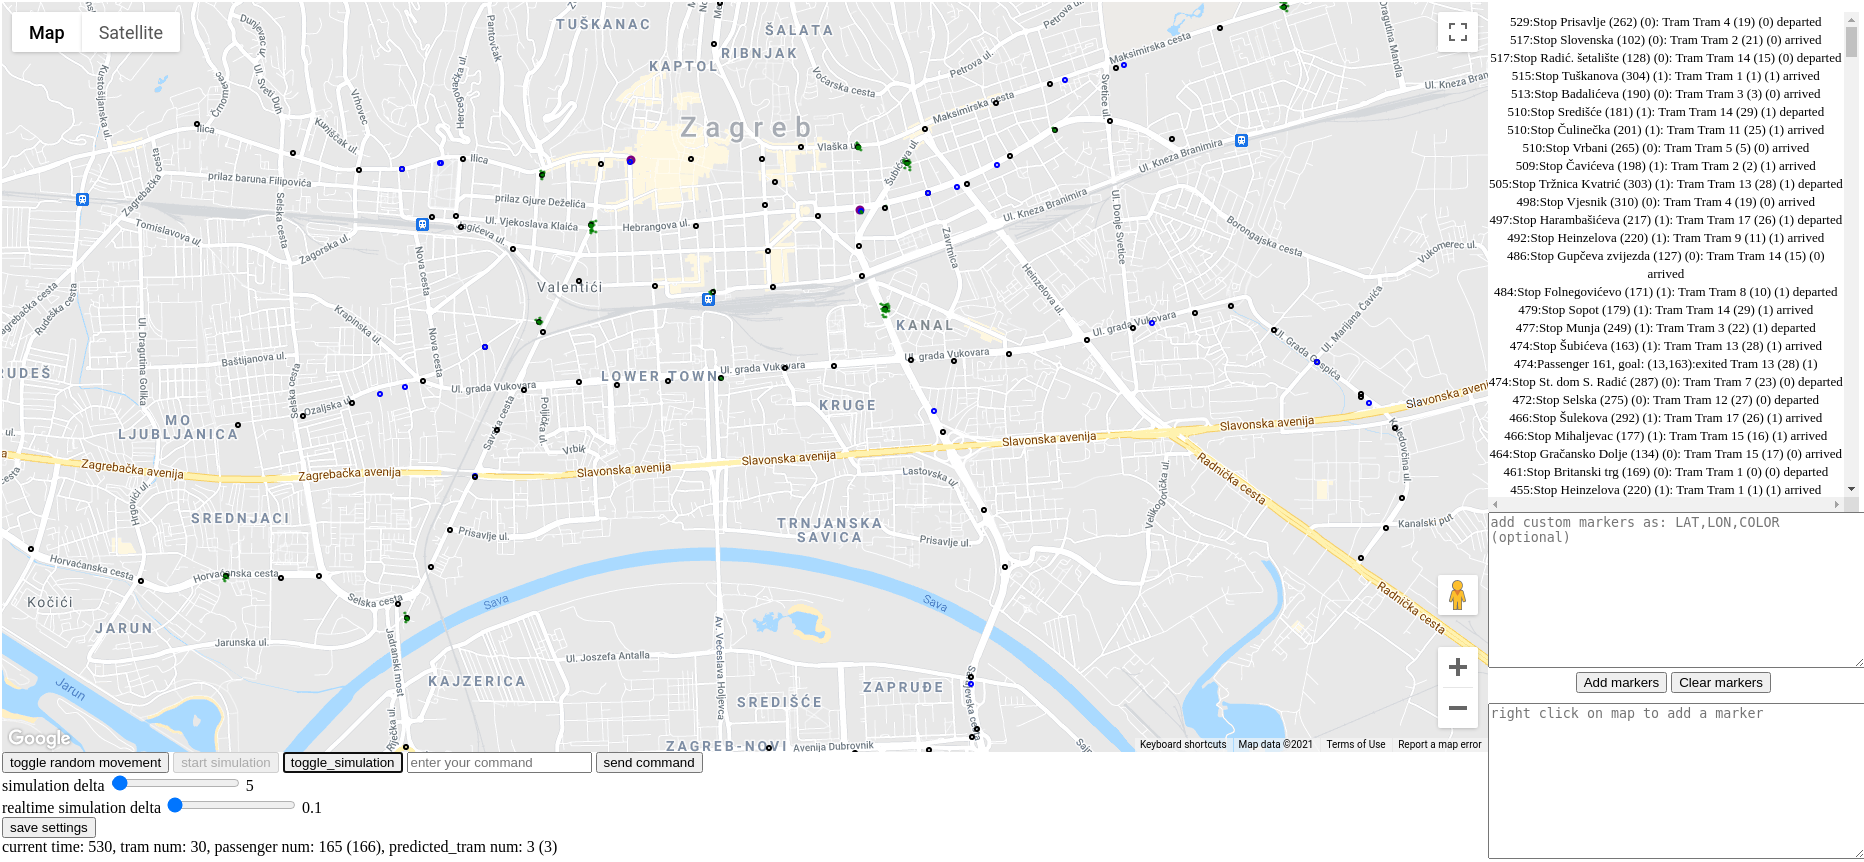
\includegraphics[width=1\textwidth]{images/frontend_full.png}
    \caption{Prikaz cijele vizualne komponente}\label{fig:frontend_full}
\end{figure}

Na slici \ref{fig:frontend_full} je prikazana cijela vizualna komponenta koja se sastoji od karte, postavki za kontrolu simulacije, dnevnik događaja te još nekoliko alata poput unosa proizvoljnih markera.\\\\\\

\begin{figure}[htb]
    \centering
    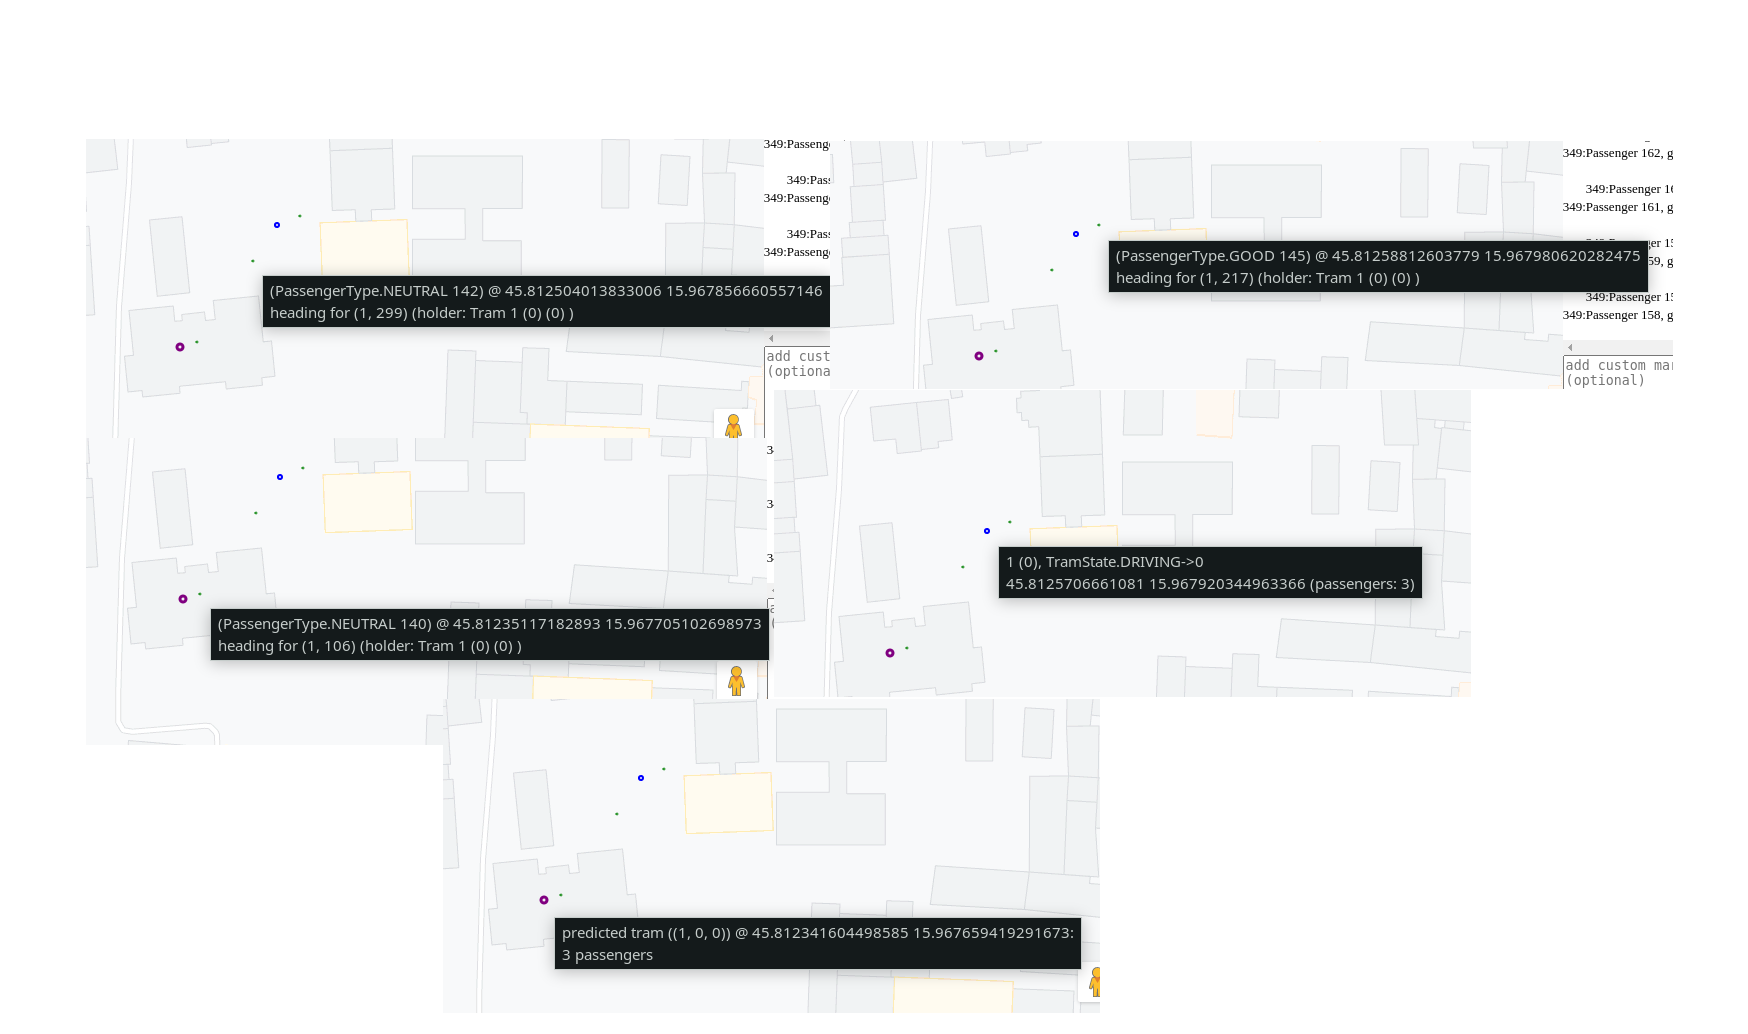
\includegraphics[width=1\textwidth]{images/frontend_group_combined.png}
    \caption{Prikaz grupe korisnika i tramvaja}\label{fig:frontend_group_combined}
\end{figure}

Na slici \ref{fig:frontend_group_combined} je prikazano 3 putnika (zelene točkice), 1 tramvaj (plava točka) te predviđeni tramvaj (ljubičasta točka). Kao što se iz slike vidi, 2 od 3 putnika su neutralni tip koji ne dijeli broj tramvaja no sustav ih i dalje (točno) grupirao.

\begin{lstlisting}[caption={Inicijalizacija karte},captionpos=b,label={kod:map_init}]
    

    

    function initMap() {
        const zagreb = { lat: 45.8, lng: 15.9819 };
        var styles = [{
            featureType: "poi",
            stylers: [
              { visibility: "off" }]}];
        map = new google.maps.Map(document.getElementById("map"), {
          zoom: 14,
          center: zagreb,
          styles: styles
        });
        google.maps.event.addListener(map, "rightclick", mapRightClick);
      }

\end{lstlisting}

Inicijalizacija karte je vrlo jednostavna, jedino što zahtjeva je \emph{API} ključ i metodu koja definira početnu lokaciju i vidljivost.

\begin{lstlisting}[caption={Pokretanje \emph{WebSocketa}},captionpos=b,label={kod:websocket_start}]
    function startSimulation() {
        socket = new WebSocket(server_address);
        socket.addEventListener('open', function (event) {
            socket.send('start_simulation');
            isSocketActive = true;
        });
        socket.addEventListener('close', function (event) {
            socket.send('simulation closed');
            isSocketActive = false;
        });
        socket.addEventListener('message', socketMessageHandler);
      }

\end{lstlisting}

Simulacija se pokreće otvaranje \emph{WebSocketa} prema \emph{backend} dijelu simulacije. Za ispravan rad je potrebno definirati metode koje se pozivaju prilikom otvaranja, zatvaranja te primanja poruka.

\begin{lstlisting}[caption={Osvježavanje markera},captionpos=b,label={kod:marker_update}]
    marker.setPosition({ lat: lat, lng: lon })
    marker.setTitle(`{lat}, ${lon}`)

\end{lstlisting}

Osvježavanje pozicije i teksta markera je također vrlo jednostavno kao što je prikazano na slici \ref{kod:marker_update}.


\subsection{Upravitelj tramvaja i tramvaji}
Upravljanje tramvajima uključuje stvaranje \engl{spawn} te pomicanje odnosno pozivanje sljedećeg koraka. Svi detalji vezani uz stvaranje se definiraju na početku simulacije. Za svaku rutu (broj tramvaja) se definira nasumičan broj vozila koji će se stvoriti te vremenski trenutak stvaranja. Zatim se ovisno o trenutnom vremenu simulacije u simulaciju ubacuju odnosno stvaraju novi tramvaji. Prilikom stvaranja se za svaki tramvaj osim same rute određuju sljedeći atributi:

\begin{itemize}
    \item index (id),
    \item početni smjer,
    \item modifikator brzine,
    \item reference na ostale upravitelje i \emph{Logger},
\end{itemize}

Osim tih, svaki tramvaja posjeduje i detalje vezane uz svoju rutu kao što su brzina putovanja između stanica koja je određena analizom datoteka ZET-a, listu stanica na ruti, itd.

Što se tiče same simulacije tramvaja, stanje tramvaja se očituje kroz sljedeće podatke:
\begin{itemize}
    \item trenutno stanje \engl{state} - može biti vožnja (\emph{DRIVING}), čekanje na stanici (\emph{STOP}), čekanje na odmorištu/okretištu (\emph{RESTING}) te zastoj (\emph{JAM});
    \item trenutna lokacija - par koordinata;
    \item redni broj zadnje obiđene stanice u ruti;
    \item trenutni vektor smjera kretanja - određen kao razlika između koordinata sljedeće i prethodne stanice;
    \item postotak pređenog puta između trenutnog para stanica - broj između 0 i 1;
    \item set putnika odnosno njihovih jedinstvenih identifikatora;
    \item preostalo vrijeme čekanja ako tramvaj nije u stanju vožnje nego u jednom od preostala 3
\end{itemize}

Glavni korak simulacije tramvaja se može opisati sljedećim, pojednostavljenim pseudokodom:

\begin{lstlisting}[caption={Glavni korak u simulaciju tramvaja},captionpos=b,label={kod:tram_main}]
    if state != DRIVING:
            remaining_time = wait()
            if state == JAM and remaining_time > 0:
                state = DRIVING
            elif state == STOP and remaining_time > 0::
                state = DRIVING
                queueManager.sign_out((current_stop_id, next_stop_id), tram_index)
                stopManager.tram_departure(current_stop_id, self)
                _set_current_info()
            else:
                if remaining_time > 0:
                    _enter_stop_state()
        else:
            jam = queueManager.jam((current_stop_id, next_stop_id), tram_index)
            if jam > 0:
                state = JAM
                current_wait_time = jam
            else:
                move()
\end{lstlisting}

U glavnom koraku simulacije pojedinog tramvaja se ovisno o trenutnom stanju događaju različite stvari. Ako tramvaj ne vozi odnosno nije u \emph{DRIVING} stanju, znači da se nalazi u jednom od preostalih stanja. Ta 3 stanja su slična po tome što imaju definirano vrijeme čekanja kao uvjet koji treba zadovoljiti prije nego što tramvaj može prijeći u sljedeće. Mogući prelasci su sljedeći:
\begin{itemize}
    \item \emph{JAM} -> \emph{DRIVING},
    \item \emph{STOP} -> \emph{DRIVING},
    \item \emph{RESTING} -> \emph{STOP},
    \item \emph{DRIVING} -> \emph{JAM},
    \item \emph{DRIVING} -> \emph{STOP},
    \item \emph{DRIVING} -> \emph{RESTING}
\end{itemize}

Ako se tramvaj nalazi u \emph{DRIVING} stanju, prvo s komponentom \emph{QueueManager} provjerava da li na trenutnom putu postoji zastoj. U slučaju da zastoja nema, poziva se metoda pomaka koja slijedi u nastavku:

\begin{lstlisting}[caption={Pomak tramvaja},captionpos=b,label={kod:tram_move}]
    tram_in_front_progress = queueManager.get_next_in_line((current_stop_id, next_stop_id), tram_index)
    distance_to_travel = current_speed * travel_time
    distance_travelled_progress = max(distance_travelled_progress + distance_to_travel, tram_in_front_progress - 0.005)
    queueManager.update((current_stop_id, next_stop_id), tram_index, min(1, distance_travelled_progress))
    if distance_travelled_progress >= 1:
        lat,lon = next_stop.latlng
        current_stop_index += 1
        distance_travelled_progress = 0.0
        passengerManager.notify_stop_arrival(set(passengers), stopManager.get_stop(next_stop_id, direction_id))
        if current_route.stops[current_stop_index] == current_route.final_stop:
            _enter_rest_state()
        else:
            _enter_stop_state()
    else:
        lat,lng = current_stop.latlng + current_direction_vector * distance_travelled_progress 
\end{lstlisting}

Pomak je napravljen kao linearna interpolacija po pravcu između 2 stanice, prethodne i sljedeće. Ono što pomak ograničava je prvi sljedeći tramvaj koji se nalaze ispred. To se provjerava preko \emph{QueueManager} komponente pozivom \texttt{get\_next\_in\_line()} metode. Ako je postotak pređenog puta manji od 1 što znači da tramvaj još nije došao do sljedeće stanice, potrebno je izračunati nove koordinate. Za to se koristi jednostavna formula:
\begin{equation} \label{formula:tram_move}
    lat,lng = currentStop.latlng + currentDirectionVector * distanceTravelledProgress
\end{equation}

S druge strane, ako je tramvaj došao do sljedeće stanice, dojavljuje svoj dolazak, prelazi u stanje ovisno da li se radi o posljednjoj stanici te kao nove koordinate uzima koordinate te stanice.

\subsection{Upravitelj zastoja i redoslijeda na pruzi}
Radi se o jednostavnoj komponenti koja za svaki par stanica i smjer (odnosno put između stanica na ruti) bilježi redoslijed tramvaja. Ovo omogućuje kontrolu da se tramvaji ne prestignu zbog razlike u brzini.
Osim toga ova komponenta na nasumičan način određuje zastoje tako da odabire određeni put između stanica (određen kao par stanica i smjer) te vrijeme čekanja. Zatim tramvaji koji su u stanju vožnje prije kretanja provjere da li se ispred njih nalazi zastoj.

\subsection{Upravitelj stanicama i stanice}
Zadatak upravitelja je omogućavanje drugim komponentama komunikaciju s određenom stanicom, određivanje na kojim stanicama će se u određenom trenutku stvarati putnici te prosljeđivanje naredbe za sljedeći korak svim stanicama. Prvi dio ovog zadatka je jednostavno napravljen tako da ova komponenta ima mapiranje između identifikatora stanica i referenci na te stanice te preko dostupnih metoda omogućuje tu komunikaciju. Drugi dio, za stvaranje putnika se svakih nekoliko koraka simulacije nasumično odabire nekoliko stanica te se na njima onda stvara nekoliko putnika kao što je prikazano sljedećim pseudokodom:

\begin{lstlisting}[caption={Stvaranje novih putnika},captionpos=b,label={kod:passenger_spawn}]
    def spawn_passengers():
        diff = passengers_active_num - max_passenger_num
        if diff < 0 or random(0,1) > 0.7 + diff / 100:
            chosen_stops = random.sample(self.spawn_viable_stops, k=5)
            for stop_id, direction_id in chosen_stops:
                stop = self.stops[(stop_id, direction_id)]
                num_to_spawn = randint(1,5)
                for _ in range(num_to_spawn):
                    passenger_goal = get_random_goal(stop_id, direction_id)
                    spawn_passenger(passenger_goal, stop_id, direction_id)

\end{lstlisting}

Kao što se može vidjeti iz koda, vjerojatnost za mogućnost stvaranja novog putnika pada ako je trenutni broj aktivnih putnika veći od ograničenja. Uz to, broj putnika koji se stvori je također nasumično određen broj između 1 i 5.

Što se tiče samih stanica, one funkcioniraju tako da u svakom koraku, ako je na stanici trenutno parkiran tramvaj, obavješćuju sve putnike koji se trenutno nalaze na njoj. Ovo znači da kao i tramvaji, stanica također posjeduje set putnika.


\subsection{Upravitelj putnika i putnici}
Upravitelj putnika radi na vrlo sličan način kao upravitelj stanica, jednostavno preko javnih metoda drugim komponentama omogućuje komunikaciju s određenim putnikom preko jedinstvenog identifikatora.

Sami putnici su jednostavni objekti koji imaju mogućnost povezati se na drugi objekt te tako odrediti svoju lokaciju. Pod drugim objektom se prvenstveno misli na stanice ili tramvaje. Osim toga, putnici komuniciraju sa sustavom za predviđanje lokacija tramvaja pritom dijeleći informacije ovisno o kakvoj vrsti putnika se radi. Zbog boljeg simuliranja stvarnog svijeta, svaki putnik ima faktor koji određuje preciznost lokacije. Radi se o jednostavnom broju između 0 i 1 koji određuje radijus nasumičnog pomaka lokacije, što je taj broj manji to je lokacija preciznija. Slijedi formula:

\begin{equation} \label{formula:passenger_location}
    location = holderLocation + accuracy * random(-0.0005, 0.0005)
\end{equation}

\texttt{holderLocation} predstavlja pravu lokaciju putnika odnosno lokaciju stanice ili vozila gdje se putnik trenutno nalazi. 


\section{Glavni tijek simulacije}
Simulacija se sastoji od 2 dijela:
\begin{itemize}
    \item \textbf{inicijalizacija} - kreiranje svih komponenti;
    \item \textbf{glavna petlja} - upravljanje komponentama i vraćanje rezultata
\end{itemize}

S obzirom na to da je većina logike smještena u same komponente, radi se o jednostavnim dijelovima. Glavna petlja se može predočiti sljedećim kodom:
\begin{lstlisting}[caption={Glavna petlja simulacije},captionpos=b,label={kod:simulation_next}]
    def next():
        logger.next_step()
        current_time += 1
        trams = tramManager.next_step()
        stopManager.next_step()
        passengers = passengerManager.next_step()
        predictedTrams = predictor.next_step()
        log = logger.pop_log()
        res = (current_time, trams, passengers, predictedTrams, log)

        return res
\end{lstlisting}



Na slici (\ref{fig:simulation_sequence_diagram}) je prikazan dijagram toka cijele simulacije. 
Radi se o malo pojednostavljenom dijagramu gdje nije prikazana sva komunikacija između komponenti. Primjerice, u sustavu komunikacija prema stanicama i putnicima ide preko upravitelja (\emph{StopManager}, \emph{PassengerManager}) no zbog smanjenja kompleksnosti je to u dijagramu prikazano direktno. \\\\\\\\\\\\\\\\\\\\

\begin{figure}[htb]
    \centering
    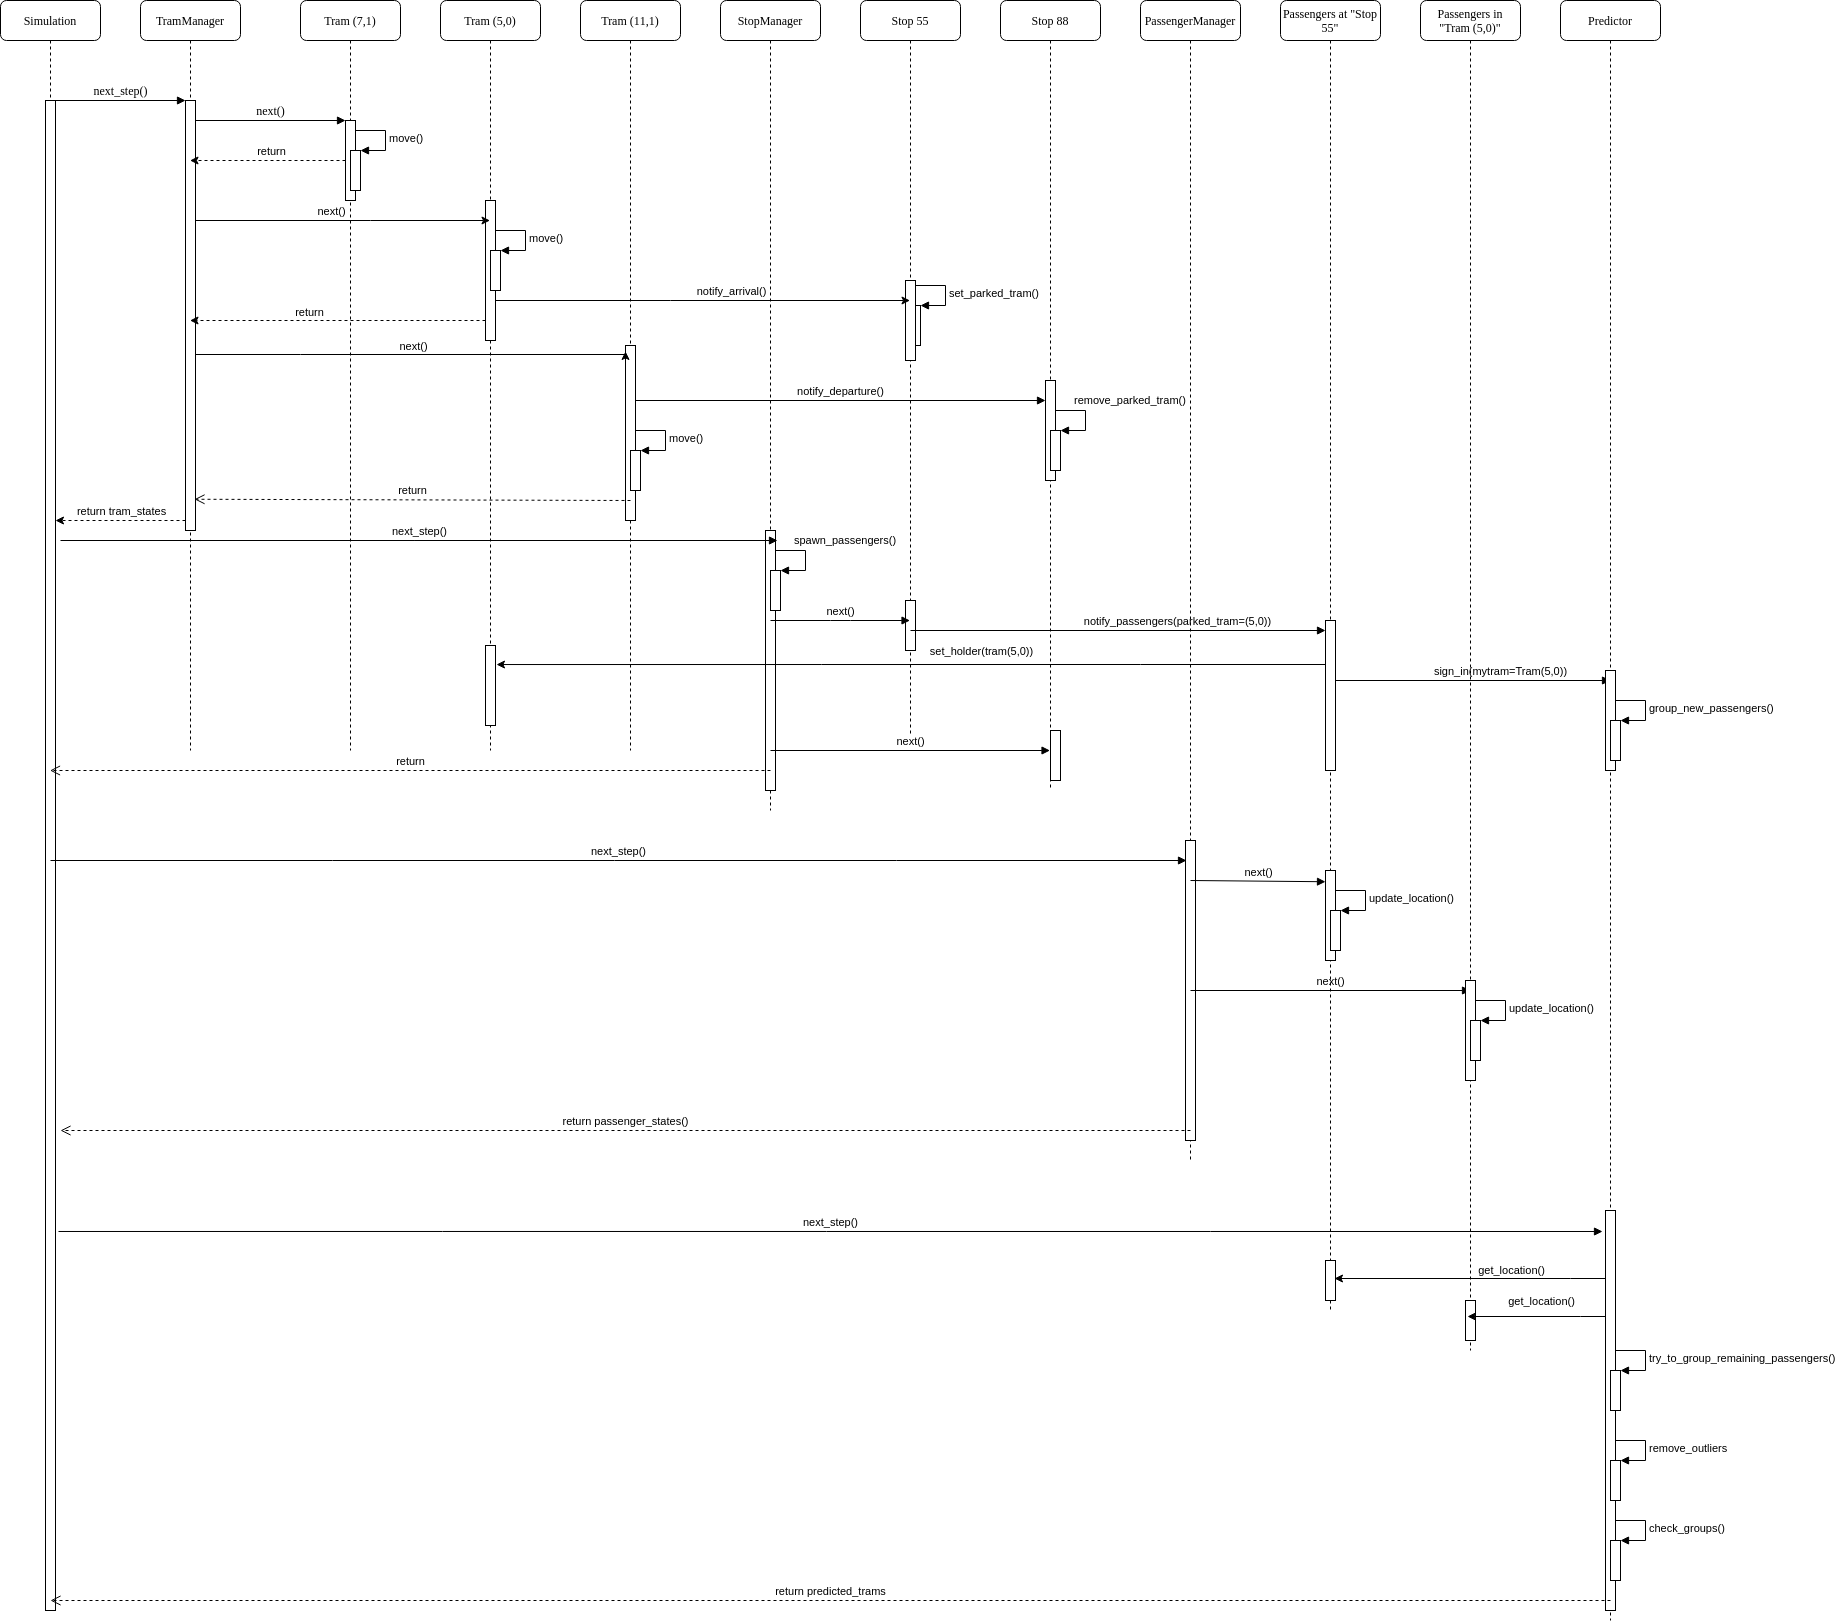
\includegraphics[width=1\textwidth]{images/simulation_sequence_diagram.png}
    \caption{Dijagram toka cijele simulacije}\label{fig:simulation_sequence_diagram}
\end{figure}


\section{Performanse simulacije}
Testiranje performansi simulacije, odnosno određenih komponenti simulacije je bilo napravljeno mjerenjem potrebnog vremena izvršavanja svakog koraka simulacije za svaku komponentu. Ovo se jednostavno izvelo iz glavne petlje simulacije. U sljedećoj tablici slijede rezultati nekoliko testova:

\begin{table}[htbp]
    \caption{Performanse simulacije}
    \label{tbl:simulacija}
    \centering
    \small
    \setlength\tabcolsep{2pt}
    \begin{tabular}{ccc|cccccc} \hline
    \thead{Koraci\\ (s)} & \thead{Broj\\ putnika} & \thead{Dobri\\ putnici \\ (\%)} & \thead{Trajanje\\ (s)} & \thead{Faktor\\ ubrzanja \\ (\%)} & \thead{Tramvaji\\ (\%)} & \thead{Stanice\\ (\%)} & \thead{Putnici\\ (\%)} & \thead{Predikcija\\ (\%)}\\ \hline
    10000 & 100 & 0 & 67 & \textbf{149} & 13.2 & 2.4 & 9.2 & 75.2 \\
    10000 & 100 & 25 & 41.3 & \textbf{242.0} & 21.7 & 4.3 & 14.9 & 59.2 \\
    10000 & 100 & 50 & 33.4 & \textbf{299.7} & 26.6 & 4.8 & 18.1 & 50.5 \\
    10000 & 100 & 75 & 22.2 & \textbf{449.9} & 39.3 & 7.3 & 27.5 & 25.9 \\
    10000 & 100 & 100 & 19.7 & \textbf{507.8} & 45.4 & 8.1 & 31.3 & 15.2 \\
    10000 & 300 & 0 & 180.5 & \textbf{55.4} & 5.0 & 1.1 & 8.6 & 85.3 \\
    10000 & 300 & 25 & 70.6 & \textbf{141.7} & 12.7 & 2.7 & 22.2 & 62.3 \\
    10000 & 300 & 50 & 47.6 & \textbf{209.9} & 19.2 & 4.1 & 33.3 & 43.4 \\
    10000 & 300 & 75 & 38.8 & \textbf{257.7} & 24.4 & 5.3 & 42.1 & 28.2 \\
    10000 & 300 & 100 & 31.7 & \textbf{315.5} & 27.7 & 5.9 & 48.6 & 17.7 \\
    10000 & 500 & 0 & 300.4 & \textbf{33.3} & 3.1 & 0.8 & 8.5 & 87.6 \\
    10000 & 500 & 25 & 126.7 & \textbf{78.9} & 7.3 & 1.8 & 20.3 & 70.5 \\
    10000 & 500 & 50 & 69.6 & \textbf{143.6} & 13.0 & 3.4 & 36.1 & 47.5 \\
    10000 & 500 & 75 & 55.7 & \textbf{179.6} & 16.4 & 4.1 & 44.8 & 34.7 \\
    10000 & 500 & 100 & 44.2 & \textbf{226.3} & 20.9 & 5.1 & 56.9 & 17.2 \\
    20000 & 300 & 0 & 408.2 & \textbf{49.0} & 5.0 & 1.0 & 7.7 & 86.3 \\
    20000 & 300 & 50 & 108.1 & \textbf{184.}9 & 18.7 & 3.6 & 29.8 & 47.9 \\
    20000 & 300 & 100 & 66.1 & \textbf{302.4} & 29.4 & 5.8 & 46.5 & 18.3 \\ \hline
    \end{tabular}
\end{table}

Trajanje simulacije ovisi o nekoliko faktora. Osim očitog, broja koraka simulacije, najbitniji su broj putnika te vrste putnika. Naime, što je u sustavu više "dobrih" putnika odnosno onih koji uz lokaciju dijele i broj/smjer tramvaja, to se komponenta predviđanja brže izvodi jer ne treba raditi česte usporedbe povijesti lokacija. Razlike se najbolje vide pomoću faktora ubrzanja odnosno omjera trajanje simulacije (koraka simulacije) te stvarnog trajanja simulacija kao što je prikazano sljedećim grafom:\\\\\\

\begin{figure}[htb]
    \centering
    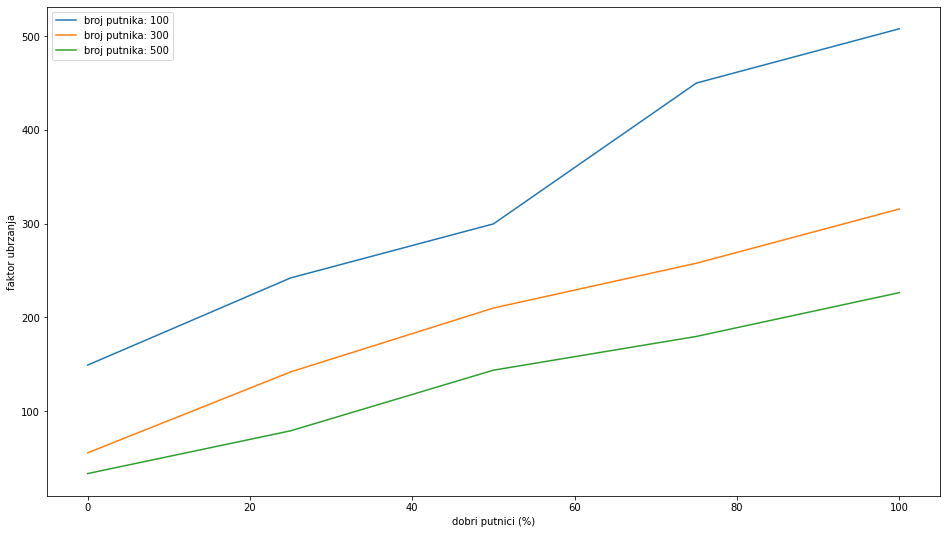
\includegraphics[width=1\textwidth]{images/simulation_performanse_graph.png}
    \caption{Faktor ubrzanja ovisno o parametrima}\label{fig:simulation_performanse}
\end{figure}


Detaljniji pogled na komponentu predviđanja u slučaju kad nema dobrih putnika otkriva sljedeću podjelu vremena izvršavanja:
\begin{itemize}
    \item osvježavanje lokacija i grupiranje putnika: 30-50\%,
    \item osvježavanje lokacija grupa/tramvaja: 30-50\%,
    \item provjera valjanosti grupa: ~20\%
\end{itemize}

Naravno utjecaj na trajanje simulacije ima i brzina procesora računala na kojemu se simulacija izvodi.

Bitno za napomenuti je kako se cijela simulacija odvija u jednoj dretvi. Višedretvenost bi mogla poboljšati performanse, pogotovo komponente za predviđanje lokacija tramvaja no pravilna implementacija bi zahtijevala potpunu promjenu logike cijelog sustava i uvođenje raznih sinkronizacijskih mehanizama što nije lagana stvar. Osim jednostavnosti, pogodnost ili boljim riječima način na koji se izvođenje na jednoj dretvi može iskoristiti, je istovremeno izvođenje nekoliko simulacija (svaka u svom procesu).

Što se tiče potrošnje radne memorije, jedan proces odnosno instanca simulacije s 500 simuliranih putnika gdje je 50\% putnika dobrog tipa troši oko 120MB radne memorije.


\section{Nedostaci simulacije}
Savršenu simulaciju je vrlo teško napraviti, pogotovo ako se radi o simulaciji sustava s potencijalno jako velikim brojem sudionika.
Razlozi nesavršenosti simulacije mogu biti razni, glavni bi bili nedovoljna količina informacija korištenih kao parametri simulacije. Primjerice, za simulaciju napravljenu za potrebe ovog rada, to su nepoznat broj aktivnih tramvaja u zadanom trenutku, lokacije semafora i sličnih faktora koji mogu uzrokovati zastoj, vjerojatnost kvara tramvaja, broj aktivnih korisnika, itd. Nedostatak informacija znači da se neki od tih faktora jednostavno ignoriraju, dok se drugi aproksimiraju.

\subsection{Kašnjenje poruka u stvarnom svijetu}
U implementaciji simulacije nije bilo problema što se tiče kašnjenja poruka jer se cjelokupna simulacija odvijala u jednom procesu. U stvarnom svijetu to ne bi bio slučaj, pogotovo kad se u obzir uzme činjenica da su glavni sudionici mobilni uređaji spojeni na pokretnu mrežu. Osim kašnjenja moguće je i da određene poruke uopće ne stignu ili da korisnici jednostavno prestanu dijeliti lokaciju u bilo kojem trenutku. Nijedan od navedenih nedostataka ne bi trebao predstavljati veliki problem. Kašnjenje poruka se jednostavno može riješiti stavljanjem poruka u red uz pamćenje vremena slanja. Komunikacija između korisnika i sustava bi najvjerojatnije bila dvosmjerna tako da niti drugi nedostatak ne bi trebao biti problem jer bi sustav jednostavno ponovno poslao zahtjev za lokacijom. U slučaju da se korisnik odspoji odnosno prekine vezu sa sustavom, jedino što treba napraviti je izbaciti ga iz grupe u kojoj je bio.

\subsection{Nepreciznost GPS-a}
Preciznost GPS-a ovisi o mnogo faktora, kao što su kvaliteta prijamnika, trenutna lokacija (utjecaj zgrada, mostova...), brzina kretanja, itd. U implementaciji simulacije je nepreciznost bila simulirana na jednostavan način kao što je prikazano formulom \ref{formula:passenger_location} odnosno nasumičnim pomicanjem lokacije u određenom radijusu. Naravno, ovo ne pokriva sve moguće probleme koji mogu nastati u stvarnom svijetu ali je dovoljno dobro za potrebe simulacije i ovog rada.


\chapter{Zaključak}
Svrha rada je bila razviti programsko rješenje odnosno algoritam koji pomoću analize korisničkih podataka otkriva trenutno stanje u prometu, specifično lokacije vozila javnog prijevoza. Za potrebe testiranje je razvijena simulacija. Rezultati su zadovoljavajući. Dodatna poboljšanja u implementaciji simulacije bi bila simuliranje korisnika izvan tramvaja, više vrsta malicioznih korisnika, dodavanje simuliranog kašnjenja poruka u simulaciji.

Naravno, sljedeći tijek u razvoju ovakvog sustava je razvoj mobilne aplikacije i pravog poslužiteljskog dijela. Ovo bi zahtijevalo daljnja testiranja, pogotovo stvari koje je bilo teško simulirati kao što su potrošnja baterija mobitela, skalabilnost, itd.

Najveći problem odnosno prepreka za rad ovakvog sustava je kako proširiti ideju te "natjerati" ljude da pomognu drugima dijeleći svoju lokaciju. Glavni razlozi zašto netko ne bi koristio ovakav sustav bi bili potrošnja baterija mobitela te činjenica da se radi o nečemu što treba ručno pokrenuti. Kad je u pitanju potrošnja baterije uzrokovana traženjem lokacije putem GPS-a, jednostavno rješenje je smanjiti učestalost dijeljenja lokacije pojedinačnog korisnika no da bi rad sustava ostao na istoj razini, ovo znači da je potrebno sudjelovanje većeg broja korisnika. Što je broj korisnika koji je voljan dijeliti lokaciju veći, to se učestalost dijeljenja lokacije pojedinog korisnika smanjuje.

S druge strane, tu je problem ručnog pokretanja usluge dijeljenja koji može dovesti do toga da osoba ponekad zaboravi, a ponekad ne želi trošiti svoje vrijeme na pokretanje usluge. Prirodno rješenje je da aplikacija cijelo vrijeme radi u pozadini te automatski dijeli lokaciju kad se detektira vožnja u vozilu javnog prijevoza. Tu se opet pojavljuje problem potrošnje baterije. 

Poticaj za sudjelovanje bi moglo biti nagrađivanje korisnika. Primjerice, kad bi sustav bio razvijen uz podršku grada ili službe za prijevoz, moguće nagrade bi bile besplatne karte za korištenje usluge prijevoza ili neke drugi benefiti koje grad može pružiti.



\bibliography{literatura}
\bibliographystyle{fer}

\begin{sazetak}
Tema rada je rješenje za problem detektiranja stanja prometa u gradskoj okolini, prvenstveno stvarnovremenskog lociranja vozila javnog prijevoza. Zamišljeno rješenje uključuje korisnike dijele svoju lokaciju te opcionalno i druge podatke poput identifikatora vozila u kojem se nalaze. Zatim sustav na temelju tih podataka određuje lokacije vozila što daljnjom analizom omogućuje određivanje vremena dolazaka na pojedine stanice. Za razliku od drugih rješenja koja bi mogla zahtijevati znatna ulaganja u gradsku infrastrukturu, jedino što ovakav sustav treba je mobilna aplikacija, poslužitelj te dovoljan broj pojedinaca koji su voljni sudjelovati. Radi se o pojmu grupnog opažanja okoline \engl{crowdsensing}. U radu su bili obrađeni problemi poput grupiranja korisnika, detekcija o kojoj se ruti radi, izbacivanje uljeza \engl{outliera} iz grupe, itd. 

Za potrebe rada je bila razvijena simulacija koja se temeljila na podacima dobivenim iz GTFS datoteka. Analizom tih datoteka se došlo do informacija kao što su vremena putovanja između parova stanica za svaki tramvaj, udaljenost između stanica, popisi tramvaja koji prometuju određenom stanicom.

Osim kretanja tramvaja, simulacija također uključuje simuliranje korisnika koji se voze tim tramvajima. Ukratko, simulacija radi tako da sekvencijalno upravlja redom tramvajima čije se kretanje simulira linearnom interpolacijom, stanicama koje zaprimaju dolaske i odlaske tramvaja te dojavljuju korisnicima i korisnicima koji se nasumično stvaraju na stanicama te čekaju određene tramvaje. Sustav za predviđanje lokacija tramvaja od korisnika dobiva samo lokaciju te opcionalno broj tramvaja i smjer te na temelju tih dobivenih podataka grupira korisnike u grupe koje predstavljaju tramvaje i povremeno provjerava ispravnost grupa. 

\kljucnerijeci{Internet stvari, Usluge suradnog opažanja okoline, Javni prijevoz}
\end{sazetak}

% TODO: Navedite naslov na engleskom jeziku.
\engtitle{Stvarnovremenska analiza podataka korisnika javnog gradskog prijevoza}
\engtitle{Real-time data analysis of public transport users}
\begin{abstract}
The topic of this paper is a solution to the problem of detecting traffic state in the urban environment, primarily the real-time location of public transport vehicles.

The imagined solution involves users sharing their location and optionally other data such as the identifier of the vehicle in which they are currently driving in. Then, based on this data, the system determines the locations of vehicles, which allows further analysis to determine the time of arrival at individual stations. Unlike other solutions that could require significant investment in the city infrastructure, the only thing such a system needs is a mobile application, a server and a sufficient number of individuals willing to participate. The name of this technique is called \emph{crowdsensing}. The paper deals with problems such as user grouping, detection of the route based on location history, detection of outliers in a group, etc.

For the purposes of this paper, a simulation based on data obtained from GTFS files was developed. The analysis of these files yielded information such as travel times between pairs of stations for each tram, the distance between stations and lists of trams running on a particular station.

In addition to the movement of trams, the simulation also includes the simulation of users riding these trams. In short, the simulation works by sequentially controlling trams which move by a method linear interpolation, stations that get notified by tram arrivals/departures and finally users who get randomly created at stations and wait for certain trams. The tram location prediction system receives only the location and optionally the tram identifier from the user, and on based on this data it groups users into groups representing trams and periodically checks the correctness of the groups.

\keywords{Internet of Things, Crowdsensing, Public transport}
\end{abstract}

\end{document}